%=====================================================================
%  IEEE journal manuscript. Compile with pdfLaTeX + BibTeX
%  Order:  pdfLaTeX -> BibTeX -> pdfLaTeX -> pdfLaTeX
%  Multimodal polysomnography: joint staging + respiratory-event detection.
%  Supervision draft: full benchmark, math formulation, expanded review.
%=====================================================================
\documentclass{ieeeaccess}
% Avoid "TeX capacity exceeded [PDF object stream buffer]" that Overleaf/TeXLive raises
% on large embedded figures. Disabling object-stream compression sidesteps the buffer.
\ifdefined\pdfobjcompresslevel\pdfobjcompresslevel=0\fi

% The class ships VOLUME 11, 2023 in the page footer. Production sets the real
% values; until then they should at least not contradict a 2026 manuscript.
\vol{14}
\def\theyear{2026}

\usepackage{cite}
\usepackage{amsmath,amssymb,amsfonts}
\usepackage{algorithmic}
\usepackage{graphicx}
% resolve figures/ locally (../figures) and on Overleaf (./figures)
\graphicspath{{../}{./}}
\usepackage{textcomp}
\usepackage{xcolor}
\usepackage{booktabs}
\usepackage{array}
\usepackage{multirow}
\usepackage{url}
\usepackage{stfloats}   % lets two-column (starred) floats sit at the bottom of a page
% allow more (and wider) floats per page so the many two-column tables place near
% their references instead of piling up after the bibliography.
\setcounter{topnumber}{3}
\setcounter{totalnumber}{5}
\setcounter{dbltopnumber}{3}
\renewcommand{\topfraction}{0.95}
\renewcommand{\bottomfraction}{0.7}


\def\BibTeX{{\rm B\kern-.05em{\sc i\kern-.025em b}\kern-.08em T\kern-.1667em\lower.7ex\hbox{E}\kern-.125emX}}
\usepackage[colorlinks=true,citecolor=blue,linkcolor=blue,urlcolor=blue,breaklinks=true]{hyperref}

% Headline numbers.
%
% FINAL MODEL (8 Sep 2026), three seeds x ten patient-independent folds:
%   neural stream  188 engineered features + frozen LaBraM embedding (200-d)
%   cardio stream  learned CNN over the raw 7-channel signal (0.155 M params)
%   temporal       BiLSTM, concat fusion, validated bypass, HMM Viterbi decode
% Source: results/revision/runs/final/final_model.json
% Previous feature-only values kept in comments so the diff is auditable.
\newcommand{\mmAcc}{0.739}   % was 0.722 (feature-only configuration)
\newcommand{\mmMf}{0.670}    % was 0.651
\newcommand{\mmK}{0.634}     % was 0.611
\newcommand{\mmAuc}{0.782}   % was 0.711
\newcommand{\mmAp}{0.419}    % was 0.337

% \stale{...} marks a number NOT yet regenerated for the final model. Red is a
% to-do list, not a style choice: every instance must be re-run or removed
% before submission.
\newcommand{\stale}[1]{\textcolor{red}{#1}}
\newcommand{\eegAuc}{0.654}
\newcommand{\noflowAuc}{0.778}

\begin{document}

\history{Date of publication xxxx 00, 0000, date of current version xxxx 00, 0000.}
\doi{10.1109/ACCESS.2026.DOI}

\title{A Physiologically Interpretable Multimodal Model for Joint Sleep Staging
and Respiratory-Event Detection in Subacute Ischemic Stroke}

\author{\uppercase{Md Wahiduzzaman Suva}\authorrefmark{1},
\uppercase{Esm-e Moula Chowdhury Abha}\authorrefmark{1},
\uppercase{Md Imtiaj Alam Sajin}\authorrefmark{1},
AND \uppercase{Md Iftekharul Mobin}\authorrefmark{1}}

\address[1]{Department of Computer Science and Engineering, American International
University-Bangladesh, Dhaka 1229, Bangladesh}

\corresp{Corresponding author: Md Iftekharul Mobin (e-mail: iftekhar.mobin@aiub.edu).}

\tfootnote{The authors received no specific funding for this work.}

\titlepgskip=-21pt

\begin{abstract}
Sleep-disordered breathing is common after an ischemic stroke and predicts
worse recovery, yet automatic sleep analysis reads only the electroencephalogram and
reports only sleep stages. The polysomnogram records far more, and here the disease
is visible in its cardiorespiratory channels: the median patient
has a scored respiratory event in $13\%$ of epochs. We present MM-Net, a two-stream
multi-task model reading fourteen neural and cardiorespiratory channels, which from one
forward pass gives the sleep stage of every 30-second epoch and a per-epoch
respiratory-event label, with a direct path carrying breathing effort to
that decision. On iSLEEPS, a stroke-specific
polysomnography corpus ($99$ patients, $92{,}560$ epochs), under patient-independent ten-fold cross-validation, MM-Net stages sleep at
$\mmAcc$ accuracy (Cohen's $\kappa$ $\mmK$) and flags the epochs carrying a
respiratory event at $\mmAuc$ AUC, an epoch-level and not event-level read-out,
with $2.76$\,M parameters. Against matched single-task models, identical but for
the loss, it leads on both tasks, and against the closest prior joint
system it leads in every fold on every metric. We benchmark thirteen architectures retrained
here and three applied zero-shot from healthy sleep; every retrained baseline lands
between $0.613$ and $0.720$ accuracy, and the five reimplementations publishing
an accuracy are recovered to within $0.04$,
placing the limit in the cohort itself. Repeating the architecture search inside the
training data, so no test patient influences the model scoring it, costs $0.006$
accuracy. On healthy sleep
the same architecture reaches $0.856$, losing $0.115$ crossing into stroke against $0.140$
to $0.148$ for those baselines. Code, features and checkpoints are released.
\end{abstract}

\begin{keywords}
Cardiorespiratory signals, feature fusion, ischemic stroke, multi-task learning,
multimodal learning, polysomnography, sleep apnea, sleep staging.
\end{keywords}

% turns on IEEEtran.bst url output, which is off by default
\bstctlcite{IEEEexample:BSTcontrol}
\maketitle

%=====================================================================


%=====================================================================
\section{Introduction}
\PARstart{S}{leep} is scored in 30-second epochs into five stages, Wake (W), N1, N2,
N3, and rapid-eye-movement (REM), following the American Academy of Sleep Medicine (AASM)
rules~\cite{aasm2023manual}. The overwhelming majority of automated methods read a single
electroencephalogram (EEG) channel and ask one question: how accurately can the five stages
be classified? Two decades of work on that question have moved from convolutional and
recurrent encoders~\cite{supratak2017deepsleepnet,phan2019seqsleepnet,supratak2020tinysleepnet}
through attention and sequence models~\cite{eldele2021attnsleep,phan2021xsleepnet,
perslev2019utime} to large self-supervised EEG foundation
models~\cite{labram2024,cbramod2025,eegpt2024,biot2023}. On healthy sleepers these methods
reach roughly $85\%$ accuracy, and recent reviews argue the field is near a ceiling set by
inter-scorer disagreement~\cite{phan2022survey,yang2026review}.

A clinical polysomnogram (PSG), however, is a recording of the whole sleeping body. It
carries the EEG, eye movements, muscle tone, the electrocardiogram (ECG), nasal and oral
airflow, thoracic and abdominal breathing effort, and peripheral oxygen saturation
(SpO$_2$). These cardiorespiratory channels are where sleep-disordered breathing shows: a paused breath, a chest that keeps straining against a closed airway, a fall in
blood oxygen, and the arousal that rescues the breath. A model that reads only the EEG
cannot see any of this, and so cannot report on the disorder that most damages a patient's
sleep. We read the polysomnogram across both neural and cardiorespiratory physiology, and we
ask a question that the staging race does not:
what does a model gain, and on which clinical task, when it reads the whole recording rather
than the brain alone.

We study this on iSLEEPS~\cite{maiti2026isleeps}, released in 2026 and described by its
authors as the first Asian and one of the largest stroke-specific sleep databases. The cohort is well matched to the question.
Sleep-disordered breathing is common in the weeks after a stroke and is tied to worse
recovery~\cite{bassetti2006sleep,denis2024sleep}, and in this corpus the median patient
carries a scored respiratory event in $13\%$ of epochs, with $79$ of $99$ patients above
$5\%$ (Fig.~\ref{fig:prev}). The cardiorespiratory signal is therefore abundant and
clinically meaningful in exactly the population where breathing matters most. The published
staging baselines on this corpus reach $74.7\%$ accuracy for an LSTM, about ten points below
the healthy state of the art, and a concurrent study reports that deep networks attend to
non-physiological regions on this cohort~\cite{bose2026gap}, so the setting also stresses
every staging architecture we can bring to it.

We present a two-stream, multi-task model that treats staging and respiratory-event
detection as one joint problem, and we place it inside a broad benchmark on the same folds. Our
contributions are:

\begin{enumerate}
\item \label{c:model}We introduce MM-Net, a two-stream multi-task model that stages sleep at $\mmAcc$
accuracy ($\kappa$ $\mmK$) and, from the same forward pass, detects respiratory events at
$\mmAuc$ AUC, with a direct cardiorespiratory path to the respiratory head so
cardiorespiratory cues reach the decision undiminished by a fusion trained mostly
for staging; removing that path costs $0.006$ respiratory AUC and leaves staging unchanged
(Section~\ref{sec:method}). Against matched single-task models differing only in the
surviving loss term, the joint objective is ahead on both outputs, by $0.006$ staging
accuracy in nine folds of ten and $0.007$ respiratory AUC in seven, so the second task is
obtained without spending the first (Section~\ref{sec:joint}). The ablation identifies respiratory effort, not oxygen
saturation, as the channel the read-out depends on (Section~\ref{sec:ablate}).

\item \label{c:bench}We benchmark the model against seventeen baseline configurations, those we ran ourselves
on the same patient-independent folds as the proposed model, covering convolutional, recurrent, attentional and fully
convolutional families, and reimplement six published architectures (U-Time,
TinySleepNet, SleepTransformer) so that every comparison runs through one pipeline
(Table~\ref{tab:bench}). Among them is the closest prior joint system,
Huttunen~et~al.~\cite{huttunen2023simultaneous}, ported from its authors' released code, and
the only baseline that scores both tasks; the proposed model is ahead of it in every fold on
every metric.

\item \label{c:ceiling}We establish that the accuracy attainable on this cohort is limited by the patients and
not by our implementations. The five reimplementations whose papers report an accuracy
recover their published Sleep-EDF
figure to within $0.04$, every retrained baseline lands between $0.613$ and $0.720$
here, and the proposed model loses $0.115$ accuracy crossing from healthy sleep to stroke
against $0.140$ to $0.148$ for those baselines (Section~\ref{sec:domaingap}).

\item \label{c:resp}We show the respiratory read-out is physiologically grounded: removing the airflow
channel from which the events were scored leaves detection at $\noflowAuc$ AUC, because
the decision rests on respiratory effort above all, together with oxygen desaturation,
cardiac variability and cortical arousals, encoded redundantly enough that no single
channel is indispensable (Section~\ref{sec:noflow}).

\item \label{c:attrib}We attribute each output to the physiology it depends on, by
intervention on the model. A
leave-one-out modality-ablation grid separates the two outputs: removing the
cardiorespiratory stream lowers respiratory detection and leaves staging untouched
($-0.128$ AUC, Wilcoxon on ten fold-means, Holm $p=0.018$), while no neural ablation
moves respiratory AUC. That double dissociation is a falsifiable account of what each
modality contributes (Table~\ref{tab:ablate}).
\end{enumerate}

Together, these results reframe the problem on this cohort: the useful gains come from reading
the whole sleeping body and attributing each output to the physiology that produces it;
deeper single-channel staging does not help on this cohort. The remainder of the paper develops the model
(Section~\ref{sec:method}) and tests each claim in turn.

%=====================================================================
\section{Related Work}
\label{sec:related}

\subsection{Single-Channel Deep Sleep Staging}
Automated staging matured on one EEG channel. DeepSleepNet paired convolutional feature
extraction with a bidirectional LSTM~\cite{supratak2017deepsleepnet}; SeqSleepNet framed the
night as sequence-to-sequence labeling~\cite{phan2019seqsleepnet}; AttnSleep introduced
attention over multi-resolution convolutions~\cite{eldele2021attnsleep}; TinySleepNet and
U-Time reduced the parameter budget while holding
accuracy~\cite{supratak2020tinysleepnet,perslev2019utime}; and XSleepNet fused raw and
spectral views~\cite{phan2021xsleepnet}. More recent backbones push this further: SleepTransformer
adds interpretability and uncertainty to an attention model~\cite{sleeptransformer2022}, L-SeqSleepNet
models whole-night cycles~\cite{lseqsleepnet2023}, ZleepAnlystNet and FlexSleepTransformer explore
separated training and flexible channel sets~\cite{jirakittayakorn2024zleep,guo2024flexsleep}, and
sleep stagers built on the linear-time state-space backbone of
Mamba~\cite{gu2023mamba} reach competitive accuracy~\cite{bitmamsleep2024}.
These models set the accuracy on healthy corpora but
depend on the cortical micro-events that stroke disturbs, which is why they transfer poorly to
patients~\cite{bose2026gap}.

\subsection{Multi-Channel and Foundation Models}
Later work reads several PSG channels. U-Sleep stages from arbitrary EEG and EOG derivations
across many cohorts~\cite{perslev2021usleep}.
Joint scoring of the two tasks is itself established. Huttunen~et~al.\ trained a single network to score sleep stages and respiratory events
simultaneously across $877$ clinical recordings, comparing signal combinations from
pulse oximetry alone up to a full montage~\cite{huttunen2023simultaneous}, and multitask
staging-and-apnea models have followed~\cite{multitask2025elderly}. Those studies work in
suspected-apnea and elderly populations; what is untested is whether the arrangement
survives a cohort whose neural signal is itself damaged, which is the question this paper
asks and which Section~\ref{sec:results} answers by running their architecture here, on
these folds, from the code they released. Foundation models such
as LaBraM, CBraMod, EEGPT, and BIOT learn transferable representations from large unlabeled
corpora~\cite{labram2024,cbramod2025,eegpt2024,biot2023}. SleepFM extends this idea to several
PSG modalities~\cite{sleepfm2026}, while cross-scale foundation models and standardized
benchmarks continue to appear~\cite{csbrain2025,neuroatlas2026,sleepyland2026}, self-supervised
pretraining is now systematically evaluated for label efficiency~\cite{estevan2025ssl}, transfer
and domain adaptation improve robustness across cohorts~\cite{guillot2023transfer}, and recent
surveys and clinical benchmarks catalogue the field~\cite{yang2026review,hanif2025insomnia}. The eye and muscle channels help most with REM and Wake,
which a single EEG channel resolves poorly. Reported gains from adding respiratory channels to
\emph{staging} are small and cohort-dependent; our benchmark quantifies this directly on a
high-burden clinical cohort and separates the staging effect from the respiratory one.

\subsection{Detection of Sleep-Disordered Breathing}
A parallel line of work detects apnea and hypopnea from breathing signals. Airflow and effort
shape, oximetry, and ECG-derived heart-rate variability are all informative, and oxygen
desaturation is part of the scoring criterion for a
hypopnea~\cite{aasm2023manual}. These detectors usually run
at fine time resolution on the raw breathing waveforms and are trained on that task alone. We
instead detect respiratory events on the staging epoch grid, jointly with staging, from a
shared representation, so that one model produces both clinical outputs and the two tasks
support each other during training.

\subsection{Sleep and Breathing After Stroke}
Sleep is both disturbed by stroke and predictive of recovery, and sleep-disordered breathing
is common in the subacute phase and linked to poorer functional
outcome~\cite{bassetti2006sleep,denis2024sleep,tellenbach2023brainstem}. Focal injury also changes
the micro-events that scoring relies on, the spindles, slow waves, and muscle
atonia~\cite{gottselig2002stroke,fernandez2019spindles,simpson2023laterality,facchin2020slowwaves,zheng2025spindles};
quantitative EEG markers such as the brain symmetry index further track hemispheric
injury~\cite{anastasi2017bsi}. A model that reports on breathing as well as stage is therefore of
direct clinical value in this population. Sleep staging on ischemic stroke itself is nascent, reported only as baselines on
the iSLEEPS corpus~\cite{maiti2026isleeps}, and no prior method addresses staging and respiratory
detection jointly, on a stroke population. Rather than set published accuracies side by side,
each measured on its own corpus and protocol, we re-run the architectures that matter on
these folds (Table~\ref{tab:bench}).

%=====================================================================
\section{Critical Gaps and Limitations of Prior Work}
\label{sec:gaps}
Three gaps run through the literature above, and each maps onto one of our contributions.
\emph{(i) Single-task, single-signal design.} Almost every staging model reads one or a few EEG
channels and predicts only the stage, while apnea detectors read breathing signals and predict
only events. Multimodal foundation models have begun to join them, SleepFM~\cite{sleepfm2026}
staging sleep and classifying apnea severity from one representation on a general population,
but per-epoch respiratory detection alongside staging has not been shown on a stroke cohort,
leaving the clinician with two
separate tools. Contribution~\ref{c:model} answers this with a single model that reads both
physiologies and produces both outputs.
\emph{(ii) Evaluation on healthy sleepers.} Staging accuracy is reported almost entirely on
healthy corpora such as Sleep-EDF~\cite{kemp2000sleepedf,goldberger2000physionet}, where deep
and foundation models reach a ceiling, while performance on focal brain injury is largely
unmeasured. Contributions~\ref{c:bench} and~\ref{c:ceiling} benchmark strong deep architectures,
and classical gradient-boosting
pipelines~\cite{chen2016xgboost,ke2017lightgbm,prokhorenkova2018catboost} on a
subacute-stroke cohort, show that the healthy-built networks collapse, and establish by reimplementation that the collapse is a property of the
cohort.
\emph{(iii) Attribution and reliability.} Interpretability is usually post-hoc and
unfalsifiable, and predictive uncertainty is seldom
modeled~\cite{angelopoulos2023conformal}.
Contributions~\ref{c:resp} and~\ref{c:attrib} answer this with a physiologically grounded, non-circular respiratory
read-out and an interventional modality-ablation that attributes each output to the channel whose physiology
is closest to it.

%=====================================================================
\section{Dataset and Preprocessing}
\label{sec:data}
iSLEEPS~\cite{maiti2026isleeps} contains overnight PSG from 100 subacute ischemic-stroke
patients (mean age $50.5$; 77 male, 23 female), scored by experts into the five AASM stages.
We exclude one recording after an audit: the data records of SN28 are byte-identical to those
of SN15, a duplication consistent with the anonymization and re-numbering the dataset authors
describe, and keeping it would place a training subject into the test fold in nine of ten fold
assignments, giving $N=99$. Both tasks use all $99$ patients: the twelve recordings that
lack at least one cardiorespiratory channel are scored with those channels zero-filled
instead of excluded, and we state which $N$ applies to each reported number. The corpus totals $92{,}560$ epochs. The stage distribution
(Table~\ref{tab:dist}) is strongly imbalanced, with N2 dominant and N1 and N3 scarce, which is
the clinical norm.

\begin{table}[t]
\caption{Stage distribution and respiratory-event prevalence in the corpus we model
($N=99$). Respiratory events occupy $16.0\%$ of all epochs, and the per-patient burden
ranges from $0$ to $60.5\%$, with $79$ of $99$ patients above $5\%$ (Fig.~\ref{fig:prev}).}
\label{tab:dist}
\centering
\begin{tabular}{lccccc}
\toprule
Stage & W & N1 & N2 & N3 & R \\
\midrule
Share (\%) & 26.6 & 10.2 & 42.3 & 8.9 & 12.1 \\
\bottomrule
\end{tabular}
\end{table}

\begin{figure}[t]
\centering
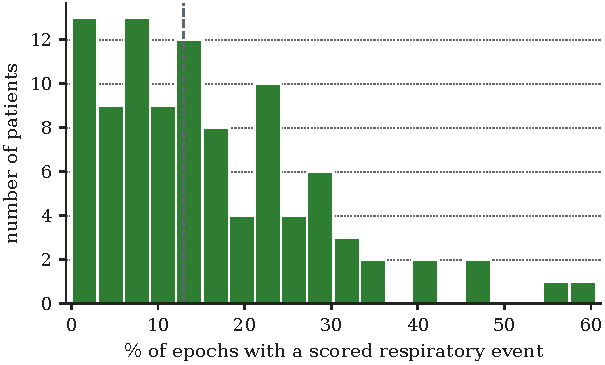
\includegraphics[width=0.86\columnwidth]{figures/fig_mm_apnea_prev.pdf}
\caption{Sleep-disordered-breathing burden across the cohort: patients by the fraction
of epochs carrying a scored respiratory event, over the $99$ with respiratory labels. The
dashed line marks the median, $13\%$.}
\label{fig:prev}
\end{figure}

\paragraph{Channels we read, and channels we do not}
A raw recording holds 22 traces. We read the 14 that carry sleep-stage or breathing
information. The \emph{neural stream} takes the four EEG derivations (C4:M1, C3:M2, O2:M1,
O1:M2), the two EOG channels (E1:M2, E2:M2), and the submental EMG. The
\emph{cardiorespiratory stream} takes the ECG, nasal and oral airflow, thoracic effort,
abdominal effort, the summed effort trace, SpO$_2$, and pulse. We leave out eight traces for
stated reasons: periodic limb movement records a different disorder; snore is scored from the
same airway sound as the respiratory events and would make the second task circular;
plethysmography is already summarized by the SpO$_2$ and pulse channels we keep; body position
is coarse and slow; and the ambient-light and battery traces are device housekeeping, not
physiology. All neural channels are resampled to $100$\,Hz for the engineered descriptors,
and independently to $200$\,Hz for the pretrained encoder as described below; the
cardiorespiratory channels go
to a common $25$\,Hz grid by polyphase resampling, which applies the anti-aliasing filter the
rate change requires; SpO$_2$, recorded natively at $4$\,Hz, is carried to this grid by the
same operation, which adds samples and no information, so
its effective resolution remains that of the $4$\,Hz oximeter. Signals are read in physical
units, which matters because SpO$_2$ near $90\%$,
pulse near $78$\,bpm, and microvolt EEG live on very different scales. Per-epoch respiratory
labels are the corpus's scored events mapped onto the $30$\,s grid, and an epoch is positive
when it overlaps an event.

%=====================================================================
\section{Proposed Method}
\label{sec:method}
\subsection{Problem Formulation}
A night is a sequence of $T$ epochs. For epoch $t$ we form a neural feature vector
$\mathbf{f}^{\mathrm{eeg}}_t\in\mathbb{R}^{388}$, formed by concatenating the $188$
engineered descriptors below with a $200$-dimensional embedding from LaBraM, a frozen
pretrained EEG encoder~\cite{labram2024} (Section~\ref{sec:repr}), and a raw cardiorespiratory tensor
$\mathbf{x}^{\mathrm{car}}_t\in\mathbb{R}^{7\times750}$, the seven channels at $25$\,Hz.
The $14$ engineered cardiorespiratory descriptors defined below are used by the baseline
configuration against which the learned encoder is measured.

The pretrained encoder is fed on its own terms. LaBraM was
pretrained at $200$\,Hz and fixes its input length at $3000$ samples, so the EEG is
resampled from our $100$\,Hz working rate to $200$\,Hz before it reaches the encoder.
Feeding the $100$\,Hz signal directly would have been silent but wrong: $3000$ samples
then span $30$\,seconds of recording while the encoder reads them as $15$, compressing
time by a factor of two, so every rhythm would present at twice its frequency and a
$12$\,Hz spindle would arrive as $24$\,Hz. At $200$\,Hz a $30$\,s
epoch no longer fits the positional embedding in one piece, so each epoch is split into
two $15$\,s sub-windows of $3000$ samples, encoded separately, and mean-pooled; the two
embeddings were checked to differ before caching, so the pooling carries information
and does not merely average duplicates. The encoder also requires canonical $10$--$20$ names
and rejects mastoid references, so C4:M1, C3:M2, O2:M1 and O1:M2 are presented as C4,
C3, O2 and O1, and the ocular and chin channels are dropped for having no canonical EEG
name. Amplitudes are scaled to $\mu$V$/100$. The encoder therefore sees four EEG
channels, strictly fewer signals than the engineered descriptors read. We learn a subject-independent
map
\begin{equation}
f_\theta:\big(\mathbf{f}^{\mathrm{eeg}}_{1:T},\mathbf{x}^{\mathrm{car}}_{1:T}\big)\ \longmapsto\
\big(\hat y^{\mathrm{stg}}_{1:T},\ \hat y^{\mathrm{apn}}_{1:T}\big),
\end{equation}
where $\Delta^4=\{p\in\mathbb{R}^5:p_k\geq 0,\ \sum_k p_k=1\}$ is the four-simplex,
$\hat y^{\mathrm{stg}}_t\in\Delta^4$ is a distribution over the five stages and
$\hat y^{\mathrm{apn}}_t\in[0,1]$ scores whether epoch $t$ contains a respiratory
event (Fig.~\ref{fig:arch}). We write $\hat y^{\mathrm{apn}}_t$ as a score and not as a
probability for the reason given in Section~\ref{sec:method}: the positive weighting in its
loss displaces the optimum away from the conditional event rate.

\begin{figure*}[t]
\centering
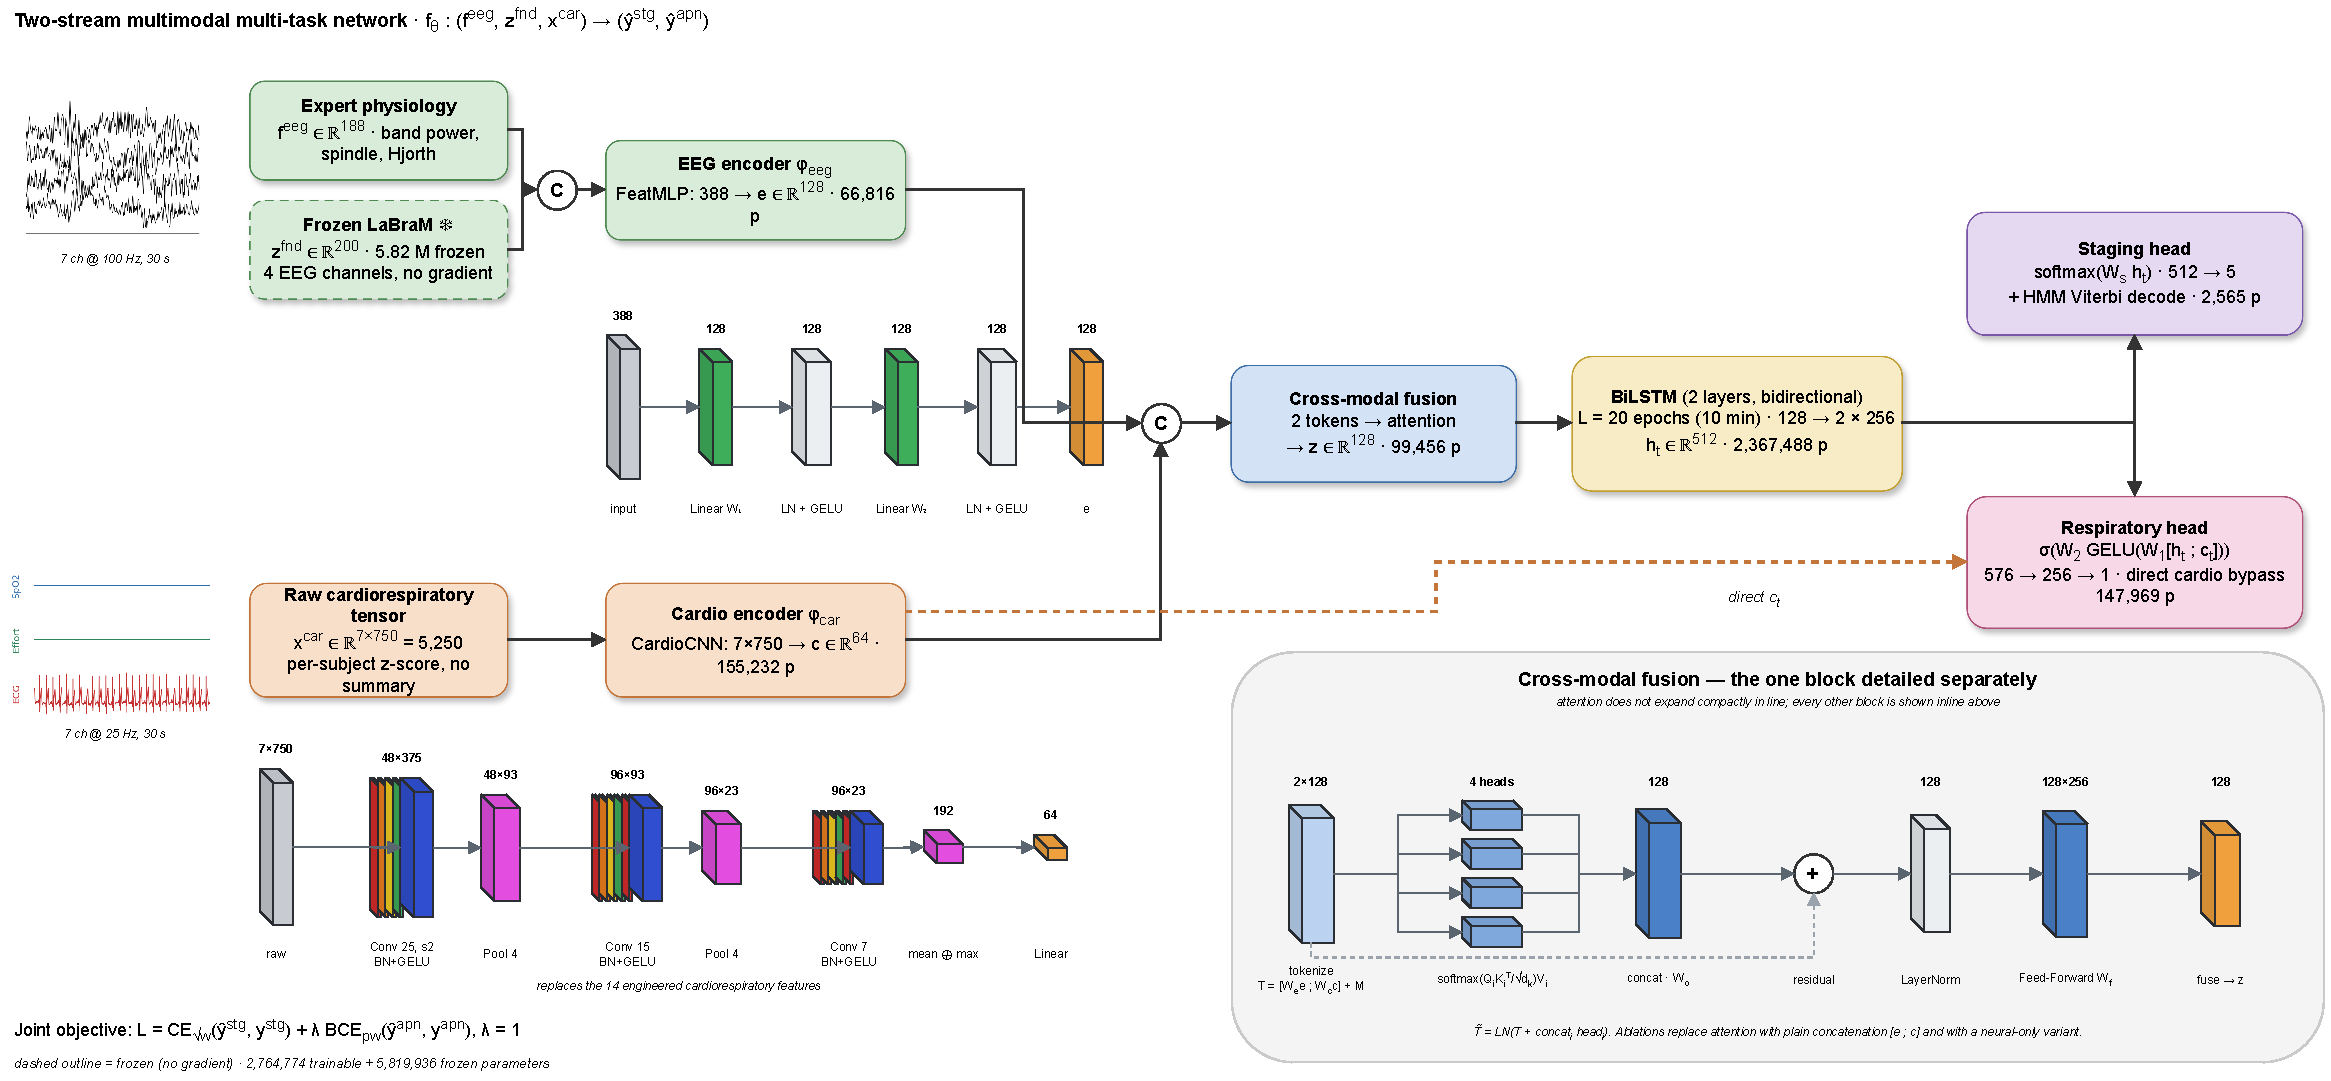
\includegraphics[width=\textwidth]{figures/fig_architecture.pdf}
\caption{The two-stream, multi-task model. Layer shapes above each block, operation
below; block height encodes units for the multilayer perceptron and temporal length for
the convolutional stack. Dashed outlines mark frozen parameters. The junction marked C is the
concatenation used for every reported result, and the fusion panel is the single linear
layer that follows it.}
\label{fig:arch}
\end{figure*}

\subsection{Physiological Feature Representations}
\label{sec:features}
\paragraph{Neural features ($188$)}
Per channel we take absolute and relative band powers from the Welch spectrum $P(f)$ in delta
($0.5$--$4$), theta ($4$--$8$), alpha ($8$--$13$), sigma ($11$--$16$), and beta
($16$--$30$)\,Hz; the relative power in band $b$ is
\begin{equation}
\mathrm{RP}_b=\frac{\int_{f\in b}P(f)\,df}{\int_{0.5}^{30}P(f)\,df}.
\end{equation}
The bands are the conventional sleep bands and alpha and sigma overlap between $11$ and
$13$\,Hz, so the five relative powers are not a partition and do not sum to one. We keep the
conventional definitions because both bands name physiology a scorer reads, and the model
treats the five as five correlated descriptors and not as shares of a whole.
We add spectral entropy $H=-\sum_i p_i\log p_i$ with $p_i$ the normalized spectrum, the
$95\%$ spectral-edge frequency, the three Hjorth descriptors~\cite{hjorth1970eeg}, and
time-domain statistics. Sleep spindles are detected on the sigma-band analytic envelope,
the modulus of the analytic signal built from the Hilbert transform $\mathcal{H}$,
$e(t)=\lvert x_\sigma(t)+i\,\mathcal{H}\{x_\sigma\}(t)\rvert=\sqrt{x_\sigma(t)^2+\mathcal{H}\{x_\sigma\}(t)^2}$, with
density counted above a per-epoch threshold. No duration, separation or morphology criterion
is applied, so this counts crossings of a sigma-band envelope and is a proxy for spindle
density and not a validated spindle detector; the same holds for the slow-wave descriptors,
which summarise amplitude and detect nothing. Ocular-movement energy on
the EOG and tonic EMG level complete the set.

\paragraph{Cardiorespiratory features ($14$)}
From the seven cardiorespiratory channels we compute SpO$_2$ mean, minimum, variability, and
desaturation depth (median minus minimum); pulse mean and variability; ECG amplitude and
line-length; airflow amplitude and line-length; thoracic, abdominal, and summed effort
amplitudes; and signed thoraco-abdominal synchrony, whose loss is the paradoxical motion of
chest against abdomen that marks an obstructed breath. The correlation is kept signed, so
synchronous and paradoxical motion sit at opposite ends of the range instead of being folded
together; a value near $+1$ is synchronous motion and a negative value is paradox,
\begin{equation}
\mathrm{sync}_t=\mathrm{corr}(x^{\mathrm{tho}}_t,\ x^{\mathrm{abd}}_t).
\end{equation}
Both feature sets are standardized per patient, which removes person-to-person offsets so the
model generalizes across people. Appendix~\ref{app:features} lists all $188$ neural
descriptors with the parameters used to compute them.

\paragraph{The learned cardiorespiratory encoder}
The evaluated model does not read the $14$ descriptors. Its cardiorespiratory branch is a
three-layer convolutional encoder over the raw $7\times750$ tensor, with wide kernels and
aggressive downsampling because respiratory events are slow: at $25$\,Hz the first kernel of
$25$ samples spans one second, and a hypopnea unfolds over $10$ to $30$. Channel widths are
$48$, $96$ and $96$, each followed by batch normalisation and GELU, with max-pooling by four
after the first two. Mean and max pooling over time are concatenated and projected by a
linear layer, LayerNorm, GELU and dropout to the same
$64$ dimensions the feature MLP produced, so the encoder is a drop-in replacement and every
other part of the network is unchanged. The branch holds $155{,}232$ trainable parameters,
of which the projection LayerNorm supplies $128$. Section~\ref{sec:repr} reports what that substitution
is worth, and it is the single largest architectural effect in this paper.

\subsection{Two-Stream Encoders}
The neural stream is a two-layer perceptron with LayerNorm; the
cardiorespiratory stream is the convolutional encoder described above, which emits a vector
of the same width the perceptron it replaced produced,
\begin{align}
e_t&=\mathrm{GELU}\!\big(\mathrm{LN}(W_2\,\mathrm{GELU}(\mathrm{LN}(W_1\mathbf{f}^{\mathrm{eeg}}_t))) \big)\in\mathbb{R}^{128},\\
c_t&=\mathrm{CardioCNN}\big(\mathbf{x}^{\mathrm{car}}_t\big)\in\mathbb{R}^{64}.
\end{align}
LayerNorm is used in place of BatchNorm because the recurrent windows are short and mix
patients within a batch, and the cardiorespiratory stream is deliberately narrower because
the branch compresses a $7\times750$ tensor into the same $64$ dimensions the
feature encoder it replaced produced, which keeps the substitution the only variable.

\subsection{Fusion}
The two embeddings are concatenated and projected back to the stream width,
\begin{equation}
z_t=\mathrm{GELU}\!\big(W_f\,[\,e_t\ ;\ c_t\,]\big)\in\mathbb{R}^{D},\qquad D=128.
\end{equation}
This is deliberately the simplest fusion available, and it is what every number in this paper
was produced with. We arrived at it by evaluating the obvious alternative first: the two
embeddings as tokens carrying learned modality-type embeddings, refined by four-head scaled
dot-product attention so each modality can read the other, then projected. On the same ten
folds, in the feature-only configuration the comparison was run in, attention was
indistinguishable from concatenation on staging ($+0.005$ accuracy, $p=0.49$) and slightly
worse on the respiratory head ($-0.014$ AUC, $p=0.06$). Since the elaborate fusion buys
nothing measurable here, we report and release the simple one, and the gain from the second
stream should be read as coming from the added modality.

\subsection{Temporal Decoder and Two Heads}
Sleep is sequential and respiratory events cluster, so the fused vectors of an $L=20$ epoch
window ($10$ minutes) are read by a two-layer bidirectional LSTM. Training draws windows at a
stride of $L/2$, so an interior epoch is seen twice per pass and an epoch in the first or last
ten of a recording once; we apply no correction for that, and the first and last window of
each night are zero-padded to $L$ under a mask that removes the padding from the loss.
Inference uses disjoint windows: a recording is padded to a multiple of $L$, split into
consecutive blocks, and the padding discarded, so every epoch is scored exactly once and no
stitching rule is needed. Hidden states are not carried between windows in either case.
Each direction runs the
standard recurrence
\begin{align}
i_t&=\sigma(W_i[z_t,h_{t-1}]), & f_t&=\sigma(W_f[z_t,h_{t-1}]),\nonumber\\
o_t&=\sigma(W_o[z_t,h_{t-1}]), & g_t&=\tanh(W_g[z_t,h_{t-1}]),\\
s_t&=f_t\odot s_{t-1}+i_t\odot g_t, & h_t&=o_t\odot\tanh(s_t),\nonumber
\end{align}
and the forward and backward states of the $256$-unit layers are concatenated into
$h_t\in\mathbb{R}^{512}$. The
staging head is a linear map $\hat y^{\mathrm{stg}}_t=\mathrm{softmax}(W_s h_t)$. The
respiratory head reads $h_t$ together with a direct copy of the per-epoch cardiorespiratory
embedding $c_t$,
\begin{equation}
\hat y^{\mathrm{apn}}_t=\sigma\!\big(W_2\,\mathrm{GELU}(W_1[h_t;c_t])\big).
\end{equation}
The connection exists so that the respiratory decision does not have to survive a
fusion trained mostly for staging, which would weaken the mechanical signature of an
obstructed breath along the way. Section~\ref{sec:ablate} identifies the channel that
signature lives in, and it is respiratory effort that names the event. We isolate the connection by removing it and holding everything else fixed, on the
same folds as every other figure here. Respiratory AUC falls from $\mmAuc$ to
$0.776$ (Wilcoxon on ten fold-means, $p=0.049$) and average precision from $\mmAp$ to
$0.411$ ($p=0.28$), while staging is untouched at $0.739$ accuracy ($p=0.92$) and $\kappa$
$0.634$ ($p=0.92$). The gain
is small, about a sixth of a fold standard deviation, and the $p$-value is marginal enough
that we would not rest an argument on it alone. What makes it worth reporting is where it
lands: the connection feeds the respiratory head and nothing
else, and the respiratory head is the only output that moves.

Removing the path is not by itself a clean test of what it carries. The head reads
$2\,\text{hidden}+d_{\mathrm{card}}$ inputs whether or not the bypass is used, because the
ablation zeroes the cardiorespiratory block instead of deleting it, so both arms hold the
same $2{,}764{,}774$ parameters and capacity is already controlled. What is not controlled
is that a head fed a constant can learn to ignore that block, which leaves open whether the
gain comes from the epoch's own breathing or merely from the presence of a plausible signal.
We therefore ran a third arm that feeds the head the same cardiorespiratory embeddings
permuted across the epochs of the window: identical capacity, identical statistics,
identical gradient path, with only the alignment to the epoch destroyed. It reaches $0.774$
AUC, which is at or just below the zeroed arm's $0.776$ and below the $\mmAuc$ of the real
path. Shuffling therefore buys nothing over zeroing, and the gain is not a capacity
artefact. We stop short of the stronger claim: against the shuffled arm the difference is
larger than against the zeroed one and yet not significant ($p=0.28$ against $p=0.049$),
because the signed test reads how consistently the folds move and not how far.

The trained model holds $2.76$ million parameters. The pretrained encoder that supplies the
$200$-dimensional neural embedding is run once offline and is not trained here, so it adds no
trainable parameters to this count.

\subsection{Training and Decoding}
The two tasks are trained together with equal weight, $\mathcal{L}=\mathcal{L}^{\mathrm{stg}}+\lambda\,\mathcal{L}^{\mathrm{apn}}$ with $\lambda=1$, combining a class-weighted staging cross-entropy and a positive-weighted respiratory cross-entropy,
\begin{align}
\mathcal{L}^{\mathrm{stg}}&=-\sum_t\sum_{k}w_k\,y^{\mathrm{stg}}_{t,k}\log\hat y^{\mathrm{stg}}_{t,k},\\
\mathcal{L}^{\mathrm{apn}}&=-\sum_t\big[\pi\,a_t\log\hat y^{\mathrm{apn}}_t+(1-a_t)\log(1-\hat y^{\mathrm{apn}}_t)\big].
\end{align}
The staging weights use the square root of inverse class frequency,
$w_k\propto\sqrt{N/(K n_k)}$ for $K=5$ classes with $n_k$ examples, which corrects the scarce
N1 and N3 stages without giving up overall accuracy, and the respiratory term is
positive-weighted by $\pi=n_-/n_+$ to match the $16\%$ event rate, which on this corpus is
$\pi\approx5.3$.

Both weightings move the optimum, and we state where. Minimising the weighted binary term
against a true conditional rate $p$ is minimised not at $p$ but at
$q^{\star}=\pi p/[\pi p+(1-p)]$, so an epoch carrying a true event probability of $0.157$ is
driven towards $0.5$; the staging weights displace the softmax by the same mechanism, to
$q^{\star}_k\propto w_k p_k$. Neither head therefore emits a calibrated posterior, and a
threshold of $0.5$ on the respiratory output is not a fifty-per-cent event probability. Both
displacements are monotone, so ranking is untouched and the AUC and average precision we
report are unaffected; what they do affect is any reading of the numbers as probabilities,
which is why Section~\ref{sec:results} treats the outputs as scores and measures calibration
separately.

At inference the staging
posteriors are smoothed by a Viterbi pass whose transition matrix $A^{\mathrm H}$
and prior are counted from the training labels~\cite{chen2024hmm},
\begin{equation}
\delta_t(j)=\max_i\big[\delta_{t-1}(i)+\log A^{\mathrm H}_{ij}\big]+\log\hat y^{\mathrm{stg}}_t(j),
\end{equation}
recovered by back-tracking, which restores the natural persistence of sleep.

This is a transition-regularised discriminative decoder and not a generative hidden Markov
model, and the distinction is worth keeping. A generative emission term is
$\log P(\mathbf{x}_t\mid s_t=j)$, whereas $\hat y^{\mathrm{stg}}_t(j)$ is a class-weighted
discriminative score computed from a bidirectional window; inserting it in the emission slot
applies the stage prior a second time, once through $A^{\mathrm H}$ and once through the
score itself. Dividing by the prior would not repair this, because the class weights and the
recurrent context have already displaced the score from any posterior it might have been.
What the pass buys is a transition prior on the output sequence, and that is what we claim
for it. The respiratory
head is left unsmoothed. Optimization uses AdamW with cosine annealing and early stopping on a
held-out set of patients.

%=====================================================================
\section{Experiments}
\label{sec:results}
\subsection{Protocol and Metrics}
All results use ten-fold, patient-independent cross-validation, so no patient appears in both
training and test, and within each training split a disjoint set of patients is held out for
early stopping. Staging is scored by accuracy, macro-F1 $\tfrac{1}{K}\sum_k\mathrm{F1}_k$, and
Cohen's $\kappa$. The respiratory task is scored by the area under the ROC curve (AUC) and
average precision (AP), which suits the $16\%$ event rate.

Every number we report is a mean over the ten folds with its standard deviation. That
standard deviation is a spread and not a confidence interval, and the distinction matters
here because the folds share training patients and are therefore dependent. The unit that
is close to independent is the patient, so we also resample patients with replacement,
$10{,}000$ times, rebuilding the pooled epoch set and recomputing every metric. That gives
$0.734$ accuracy with a $95\%$ interval of $[0.717,\ 0.750]$, $\kappa$ $0.628$
$[0.604,\ 0.651]$, respiratory AUC $0.778$ $[0.752,\ 0.802]$ and average precision $0.419$
$[0.355,\ 0.480]$. These condition on the fitted procedure: they carry the variation in
which patients were recorded and not retraining variability, and they say nothing about the
selection optimism measured below. The
folds are fixed across all configurations so that comparisons are paired. Fixing them buys
paired comparisons at a price we should state plainly: the configuration reported here was
chosen by comparing forty-nine candidates on these same ten folds, so the folds that
selected the model are the folds that score it, and the in-domain figures are not free of
selection optimism. Rather than bound it we measured it, by running the selection again
inside the training data (Section~\ref{sec:nested}): five outer patient-independent folds,
all forty-nine candidates compared on three inner folds within each outer training set, and
the winner scored once on outer patients that took no part in choosing it. That procedure
reaches $0.734 \pm 0.009$ accuracy against the $\mmAcc$ reported here, so the optimism in
the headline figure is $0.006$, about a third of the fold-to-fold standard deviation of
$0.019$. The external corpora in Section~\ref{sec:external} took no part in selection
either, so the zero-shot figures there were never exposed to it. The proposed
model, its ablations and the six reimplemented literature models all use the full ten; the
earlier retrained baselines were run at five, which Table~\ref{tab:bench} states per row. Because a single
training seed can flatter a result, we retrained the headline configuration under three
seeds on the same folds. Staging accuracy varies by $0.005$ across seeds against
$0.020$ across folds, and respiratory AUC by $0.001$ against $0.038$: fold-to-fold spread
is four times the seed spread for staging and thirty times it for respiratory detection.
The uncertainty in these results is therefore dominated by which patients fall in which
fold, which is a property of a cohort this size. Every headline figure in this paper is the mean over all thirty fold-values, ten
folds by three seeds. Paired tests, however, are computed on the ten fold-means: the three
seeds within a fold train and test on the same patients, so they are three re-rolls of one
experiment and not three independent observations, and treating them as thirty would triple
the effective sample and shrink every $p$. One consequence is worth stating plainly. With
ten paired folds the smallest two-sided Wilcoxon $p$ is $2/2^{10}=0.002$, reached when every
fold moves the same way, so after Holm correction across a family of nine the floor is
$0.018$. Several effects below sit at that floor and differ in size by more than an order of
magnitude; the test cannot separate them, and the effect sizes are reported beside every
$p$ for that reason. The three seed means for respiratory AUC are
$0.781$, $0.783$ and $0.781$, so $\mmAuc$ is stable to the third decimal under reseeding.

\subsection{Selection Inside the Training Data}
\label{sec:nested}
The figures above are produced by a configuration chosen on the folds that score it. To find
out what that is worth we ran the whole selection again with the test patients quarantined:
five outer patient-independent folds; inside each outer training set, three inner folds; all
forty-nine candidates of the original search compared on those inner folds alone; and the
inner winner retrained on the full outer training set and scored once on the outer patients.
No outer patient influences the choice of the model that scores them, so the resulting number
estimates the whole procedure, search included, instead of a configuration that already knew
its test set.

The procedure reaches $0.7336 \pm 0.0089$ accuracy across the five outer folds against
$\mmAcc$ for the reported model, so selection is worth $0.006$ accuracy here. That is about a
third of the fold-to-fold standard deviation and close to the $0.004$ the spread of the top
ten candidates suggested, which is the more useful statement: the bound we could compute
without a nested loop turned out to be roughly the right size.

What the inner loop chose is worth reporting, because it is not what the paper reports. Every
outer fold kept the neural side of the published model, the engineered descriptors with the
frozen encoder, the BiLSTM, and the same width and regularisation, and every one of them
replaced the cardiorespiratory encoder. Four selected a randomly initialised time-series
encoder over the raw signal and the fifth a random projection of the fourteen engineered
descriptors. The search therefore does not recover the learned convolutional encoder the
paper adopts, and we should not pretend otherwise.

Two things keep that from undermining the result. Whatever the inner loop picked, the outer
accuracy lands within $0.006$ of the published figure, so the choice of cardiorespiratory
encoder is not what the accuracy rests on; and this is the same conclusion
Section~\ref{sec:repr} reaches from the other direction, where a random expansion of the same
fourteen numbers recovers most of the gap to the learned encoder. The honest reading is that
the \emph{representation} of the cardiorespiratory stream matters, which is the claim
Section~\ref{sec:repr} makes, while the particular encoder that implements it does not
separate from its random counterparts at this cohort size. A reader should take the headline
accuracy as a figure that survives selection being done properly, and should not take the
learned encoder as a component this search can justify.

Two limits. Five outer folds are fewer than the ten used everywhere else, so this estimate is
noisier than the figures it is compared against; and it uses a single seed, because five
outer folds by forty-nine candidates by three inner folds is already seven hundred and
thirty-five trainings.

\subsection{Implementation and Hyperparameters}
The model is implemented in PyTorch and trained on a single NVIDIA RTX~2060 GPU (6\,GB) under
Windows. Every run is seeded, so each is individually reproducible; headline figures
average three seeds ($42$, $1$, $7$) over the ten folds, giving the thirty fold-values used
throughout. Where a result is derived from stored predictions without retraining, it comes
from the seed-$42$ run, and the text says so at that point.
Table~\ref{tab:hyper} lists the training configuration, which is identical across all folds
and every ablation, so that reported differences come from the model. The six reimplemented
baselines are trained at the optimiser, batch size and schedule of their own papers, since
imposing our settings on them would understate architectures tuned for other choices.

\begin{table}[t]
\caption{Training configuration of the proposed model, shared across all folds and every
ablation. Each reimplemented baseline is trained at its own published settings instead.}
\label{tab:hyper}
\centering
\small
\begin{tabular}{ll}
\toprule
Setting & Value \\
\midrule
Framework / hardware & PyTorch, NVIDIA RTX~2060 (6\,GB) \\
Optimizer & AdamW \\
Learning rate & $3\times10^{-4}$ \\
Weight decay & $1\times10^{-4}$ \\
LR schedule & cosine annealing \\
Sequence length $L$ & $20$ epochs ($10$\,min) \\
Batch size & $32$ \\
Max epochs / patience & $45$ / $8$ \\
Gradient clipping & $5.0$ \\
Staging class weights & $\sqrt{}$ inverse-frequency \\
Respiratory pos.\ weight & $\pi=n_-/n_+$ \\
Loss balance $\lambda$ & $1.0$ \\
Staging post-processing & HMM Viterbi smoothing \\
Cross-validation & $10$-fold, patient-independent \\
Random seeds & $42$, $1$, $7$ \\
\bottomrule
\end{tabular}
\end{table}

\subsection{Compared Methods}
We compare the model against deep networks evaluated on the same folds: convolutional and
recurrent networks trained from scratch (DeepSleepNet, AttnSleep, a four-channel CNN--BiLSTM),
six further published architectures we reimplemented for this comparison (U-Time, a
fully convolutional encoder--decoder; TinySleepNet, a compact convolutional--recurrent model;
and SleepTransformer, a purely attentional one), a
network transferred from Sleep-EDF, and a raw-signal convolutional network on all $14$ channels,
alongside the published single-channel baselines for the corpus~\cite{maiti2026isleeps}. All numbers are
patient-independent, ten-fold except for the earlier retrained baselines at five, at the hidden-Markov operating point where a model provides one.

\begin{table}[t]
\caption{Reimplementation check for the models marked $^{\dagger}$ in
Table~\ref{tab:bench}: ten-fold subject-independent cross-validation on the
Sleep-EDF Cassette subjects $0$--$20$, $40$ recordings, single Fpz-Cz derivation.
Every row compares accuracy except $^{\S}$U-Time, whose paper reports macro-F1 and no
accuracy for Sleep-EDF; that row therefore compares macro-F1 to macro-F1, and our U-Time
reaches $0.791 \pm 0.062$ accuracy, a quantity its paper does not state. Each published figure
follows its own paper's Sleep-EDF protocol, which differs in subset and split.}
\label{tab:reimpl}
\centering
\begin{tabular}{@{}l c c c@{}}
\toprule
Model & Published & Ours & $\Delta$ \\
\midrule
U-Time~\cite{perslev2019utime}$^{\S}$ & 0.79 & $0.660 \pm 0.054$ & $-0.130$ \\
TinySleepNet~\cite{supratak2020tinysleepnet} & 0.854 & $0.824 \pm 0.045$ & $-0.030$ \\
SleepTransformer~\cite{sleeptransformer2022} & 0.814 & $0.823 \pm 0.033$ & $+0.009$ \\
1D-ResNet-SE-LSTM~\cite{li2023resnetselstm} & 0.864 & $0.832 \pm 0.036$ & $-0.032$ \\
Micro SleepNet~\cite{liu2023microsleepnet} & 0.828 & $0.800 \pm 0.041$ & $-0.028$ \\
AT-BiLSTM~\cite{fu2021atbilstm} & 0.838 & $0.835 \pm 0.046$ & $-0.003$ \\
\bottomrule
\end{tabular}
\end{table}

\begin{table*}[t]
\caption{Sleep staging on iSLEEPS, patient-independent, against every architecture we
evaluated. Cells are mean $\pm$ SD across folds where per-fold values were retained.
$^{\dagger}$ marks a model we reimplemented and checked against its published Sleep-EDF
figure (Table~\ref{tab:reimpl}), $^{\ddagger}$ one
quoted from the corpus paper on its own protocol, ``feat'' engineered features.
$^{\ast}$ marks the one architecture ported from its authors' released code rather than
reimplemented from a paper; it carries no row in Table~\ref{tab:reimpl} because that paper
reports no Sleep-EDF figure to check against, and it is the only baseline here that scores
both tasks. Bold marks
the best value among rows run under our protocol.}
\label{tab:bench}
\centering
\begin{tabular*}{\textwidth}{@{\extracolsep{\fill}} l l c c c c c @{}}
\toprule
 & & & Healthy & \multicolumn{3}{c}{iSLEEPS (stroke)} \\
\cmidrule(lr){4-4}\cmidrule(lr){5-7}
Model & Input & Params\,$\downarrow$ & Acc & Acc\,$\uparrow$ & Macro-F1\,$\uparrow$ & $\kappa$\,$\uparrow$ \\
\midrule
\multicolumn{7}{@{}l}{\emph{Deep networks, retrained on iSLEEPS}}\\[1pt]
LSTM, our reimplementation$^{\dagger}$ & 1\,EEG\,$+$\,EOG & $1.16$\,M & --- & $0.720 \pm 0.032$ & $0.626 \pm 0.028$ & $0.599 \pm 0.043$ \\
CNN-ResNet18~\cite{bose2026gap}$^{\ddagger}$ & 1\,EEG\,$+$\,EOG & $\sim$11\,M & --- & 0.617 & 0.544 & 0.480 \\
DeepSleepNet~\cite{supratak2017deepsleepnet}  & 1\,EEG  & $\sim$21\,M  & --- & $0.615 \pm 0.026$ & $0.567 \pm 0.031$ & $0.483 \pm 0.038$ \\
U-Time~\cite{perslev2019utime}$^{\dagger}$ & 1\,EEG & $1.07$\,M & $0.791 \pm 0.062$ & $0.646 \pm 0.064$ & $0.524 \pm 0.057$ & $0.506 \pm 0.082$ \\
AttnSleep~\cite{eldele2021attnsleep}          & 1\,EEG  & $\sim$0.5\,M & --- & $0.716 \pm 0.042$ & $0.600 \pm 0.043$ & $0.593 \pm 0.058$ \\
TinySleepNet~\cite{supratak2020tinysleepnet}$^{\dagger}$ & 1\,EEG & $1.45$\,M & $0.824 \pm 0.045$ & $0.676 \pm 0.050$ & $0.587 \pm 0.034$ & $0.548 \pm 0.062$ \\
SleepTransformer~\cite{sleeptransformer2022}$^{\dagger}$ & 1\,EEG & $2.79$\,M & $0.823 \pm 0.033$ & $0.683 \pm 0.026$ & $0.602 \pm 0.030$ & $0.555 \pm 0.032$ \\
1D-ResNet-SE-LSTM~\cite{li2023resnetselstm}$^{\dagger}$ & 1\,EEG & $0.65$\,M & $0.832 \pm 0.036$ & $0.708 \pm 0.038$ & $0.631 \pm 0.033$ & $0.592 \pm 0.050$ \\
Micro SleepNet~\cite{liu2023microsleepnet}$^{\dagger}$ & 1\,EEG & $0.03$\,M & $0.800 \pm 0.041$ & $0.647 \pm 0.049$ & $0.558 \pm 0.028$ & $0.510 \pm 0.055$ \\
AT-BiLSTM~\cite{fu2021atbilstm}$^{\dagger}$ & 1\,EEG & $0.92$\,M & $0.835 \pm 0.046$ & $0.692 \pm 0.040$ & $0.612 \pm 0.030$ & $0.570 \pm 0.051$ \\
CNN\,+\,BiLSTM                                & 4\,EEG  & $\sim$0.6\,M & --- & $0.613 \pm 0.040$ & $0.565 \pm 0.034$ & $0.485 \pm 0.048$ \\
Sleep-EDF transfer                            & 4\,EEG  & $\sim$0.6\,M & --- & $0.623 \pm 0.020$ & 0.582 & 0.488 \\
Raw multimodal CNN                            & 14\,ch  & 0.95\,M      & --- & $0.654 \pm 0.033$ & $0.610 \pm 0.022$ & $0.544 \pm 0.037$ \\
Huttunen~et~al.~\cite{huttunen2023simultaneous}$^{\ast}$ & 4\,ch & $3.80$\,M & --- & $0.599 \pm 0.060$ & $0.495 \pm 0.067$ & $0.440 \pm 0.078$ \\
\addlinespace[2pt]\midrule
\multicolumn{7}{@{}l}{\emph{Trained on healthy sleep, applied zero-shot}}\\[1pt]
CNN                                           & 4\,EEG  & $0.49$\,M    & $0.806 \pm 0.001$ & $0.307 \pm 0.016$ & $0.223 \pm 0.013$ & $0.102 \pm 0.010$ \\
CNN\,+\,BiLSTM (CRNN)                         & 4\,EEG  & $1.15$\,M    & $0.828 \pm 0.005$ & $0.312 \pm 0.012$ & $0.253 \pm 0.006$ & $0.127 \pm 0.022$ \\
StagingSeqNet                                 & 4\,EEG  & $1.08$\,M    & $0.855 \pm 0.001$ & $0.306 \pm 0.009$ & $0.230 \pm 0.014$ & $0.091 \pm 0.015$ \\
\addlinespace[2pt]\midrule
\multicolumn{7}{@{}l}{\emph{Proposed feature-based multi-task model}}\\[1pt]
MM-Net (neural only)              & 7\,ch feat  & 2.62\,M & --- & $0.741 \pm 0.017$ & $0.668 \pm 0.020$ & $\mathbf{0.635 \pm 0.022}$ \\
\textbf{MM-Net (neural + cardio)} & 7\,ch feat $+$ raw & 2.76\,M & --- & $0.739 \pm 0.020$ & $\mathbf{0.670 \pm 0.020}$ & $0.634 \pm 0.024$ \\
\addlinespace[2pt]\midrule
\multicolumn{7}{@{}l}{\emph{Same model, healthy sleep}}\\[1pt]
MM-Net (neural only)              & 2\,EEG feat & 2.62\,M & $\mathbf{0.856 \pm 0.027}$ & --- & --- & --- \\
\bottomrule
\end{tabular*}
\end{table*}

\subsection{Staging Benchmark and Comparison}
The row marked $^{\ddagger}$ is quoted from the corpus paper and was not run here. It
uses that paper's protocol, an $80/10/10$ patient-wise split over $N=100$ that includes the
duplicated pair we exclude (Section~\ref{sec:data}), and its own two-channel input, and that
paper's repository releases preprocessing only, so it can be neither reproduced nor read as
a same-protocol comparison. Each reimplementation is checked against the figure its own paper
publishes on Sleep-EDF (Table~\ref{tab:reimpl}); those figures follow each paper's own protocol, which
differs in subset and split, so they are consistency checks.
Our own split uses one subject more than the conventional Sleep-EDF-20 set, and one of the
published figures is measured on SHHS, so those two checks are weaker
than the rest. A third is weaker still. U-Time publishes macro-F1 and not accuracy, so its
row is the only one compared in macro-F1, and there our reimplementation sits $0.130$ below
the published figure. Macro-F1 is governed by N1, the stage whose prevalence moves most
between Sleep-EDF subsets, and the published figure comes from the $39$-recording subset
under twenty-fold cross-validation against our $40$ recordings under ten, so the gap is not
readable as a failure of the reimplementation; it is readable as a comparison we cannot make
cleanly, and we mark it as such instead of converting one metric into the other.
Table~\ref{tab:bench} is organised in three blocks: architectures retrained on this
cohort, architectures trained on healthy sleep and applied to it zero-shot, and the
proposed model, with a final row cross-validating the proposed architecture on healthy
sleep as a control on the cohort argument; its macro-F1 and $\kappa$ are healthy-sleep
figures and so are left out of the stroke columns, and quoted in the text instead.
Dispersion is reported wherever it is defined: five folds for the earlier retrained
baselines; thirty fold-values, ten folds by three seeds, for AttnSleep, the three
reimplemented literature models and the proposed rows. CNN-ResNet18 is quoted from the
corpus paper and was not re-run here, so its protocol is that paper's and it
carries no interval. That paper's LSTM appears only as our reimplementation of it on the
folds used throughout, because its published figure was never measured on these folds. In the zero-shot block the interval is across
pretraining seeds and not folds, because that evaluation is a single pass of a finished
checkpoint over all $99$ patients. The two best healthy scores, $0.856$ and $0.855$, are
separated by less than either interval. Sleep-EDF carries none of the cardiorespiratory
channels this model reads, its Cassette recordings providing an oronasal airflow trace at
$1$\,Hz but no ECG, effort belts or oximetry and no scored respiratory events, so every
healthy-sleep figure exercises the neural branch alone and the comparison row there is
MM-Net (neural only).

Table~\ref{tab:bench} shows a clear pattern: every deep network, whether trained from scratch,
transferred from healthy sleep, or applied to the raw multichannel signal, stays between $0.61$
and $0.72$ accuracy, $12$ to $20$ points below the same architectures' published accuracy on
healthy sleepers. The feature-based model reaches $\mmAcc$, above every deep architecture we
retrained here, which matches the concurrent finding that depth alone does not help on this
cohort~\cite{bose2026gap}: with under a hundred patients a convolutional network cannot
rediscover what decades of sleep science already encode in the features. The corpus paper's own recurrent
baseline, reimplemented here and run on the same folds, reaches $0.720 \pm 0.032$ over
thirty fold-values. Staging accuracy is nonetheless capped: nothing we have run on this
corpus exceeds $0.75$. Section~\ref{sec:curve} shows why: the
staging learning curve has flattened, which points at the cohort and not at any one model.
We therefore do not position the model as a staging leader. What sets it apart is
a second output. Of the models that stage competitively here it is the only one that also
detects respiratory events; the raw multimodal CNN produces both outputs but stages at
$0.654$.

The comparison that speaks to this directly is against Huttunen~et~al., the closest prior
system: one network scoring sleep stages and respiratory events at once, which makes it the
only baseline in Table~\ref{tab:bench} that answers the same two questions this model does.
We ported the architecture from the authors' released code and not from the paper, so the
encoder blocks, the squeeze-and-excitation ratios, the atrous pyramid at the bottleneck and
the shape of the two segment classifiers are theirs. On the same folds it reaches
$0.599$ accuracy and $0.710$ respiratory AUC against $\mmAcc$ and $\mmAuc$, and the
proposed model is ahead in all ten folds on every metric (Wilcoxon on fold-means, $p=0.002$,
the floor at this sample size).

That margin should be read as a statement about this corpus and not about their result.
Their model was built for, and reported on, $877$ suspected-obstructive-sleep-apnea
recordings; three things had to change to bring it here. iSLEEPS has no oronasal
thermocouple, so it reads four of the five signals of their fullest configuration; their
respiratory output is a three-way decision every second, which this corpus cannot supply and
which we replaced with the same per-epoch binary label used throughout; and a single EEG
derivation at their $32$\,Hz is a thin neural input for staging, which is most of why the
staging gap is wider than the respiratory one. What the row supports is that a joint
architecture tuned on a general sleep-apnea population does not transfer to a stroke cohort
of this size, which is the same conclusion the rest of Table~\ref{tab:bench} reaches for
single-task architectures.

A representative held-out night is
shown in Figure~\ref{fig:hypno}: the predicted hypnogram follows the reference through the
night's cycles, and the stage-probability ribbon exposes where the model is confident and where
it hesitates.

The margin over the retrained baselines is tested. The folds are fixed
across every model in Table~\ref{tab:bench}, so each baseline is scored on exactly the patients
the proposed model was and the comparison is paired. That matters here: fold-to-fold variation
is large and it is \emph{shared}, because the difficulty lies in the patients (AttnSleep spans $0.627$ to $0.755$ across folds), so reading two overlapping
$\pm$SD intervals charges the cohort's own variability against the difference and hides it.
Paired on the ten fold-means, with Holm correction across the eight baselines we ran
ourselves, the proposed model is ahead of every one of them on accuracy, by $+0.019$ to
$+0.093$, and wins between eight and ten of the ten folds in each comparison. The margin is
statistically separable for five: Micro SleepNet, SleepTransformer, U-Time, AT-BiLSTM and
TinySleepNet (Holm $p$ from $0.016$ to $0.039$). For the three closest it is not. AttnSleep
($+0.023$, Holm $p=0.17$), our reimplementation of the corpus LSTM ($+0.019$, $p=0.17$) and
1D-ResNet-SE-LSTM ($+0.032$, $p=0.15$) sit inside the noise that ten folds can resolve. We
report that as it stands, and it is the cohort-ceiling argument arriving by another route:
three architectures spanning 2021 to 2023 land close enough to the proposed model that this
cohort cannot tell them apart.
The accuracy margin is the narrowest of the three and the one most exposed to the cohort's
noise; macro-F1 and $\kappa$, which do not let a model coast on the two majority stages,
separate the models by two to three times as much.

\begin{figure*}[t]
\centering
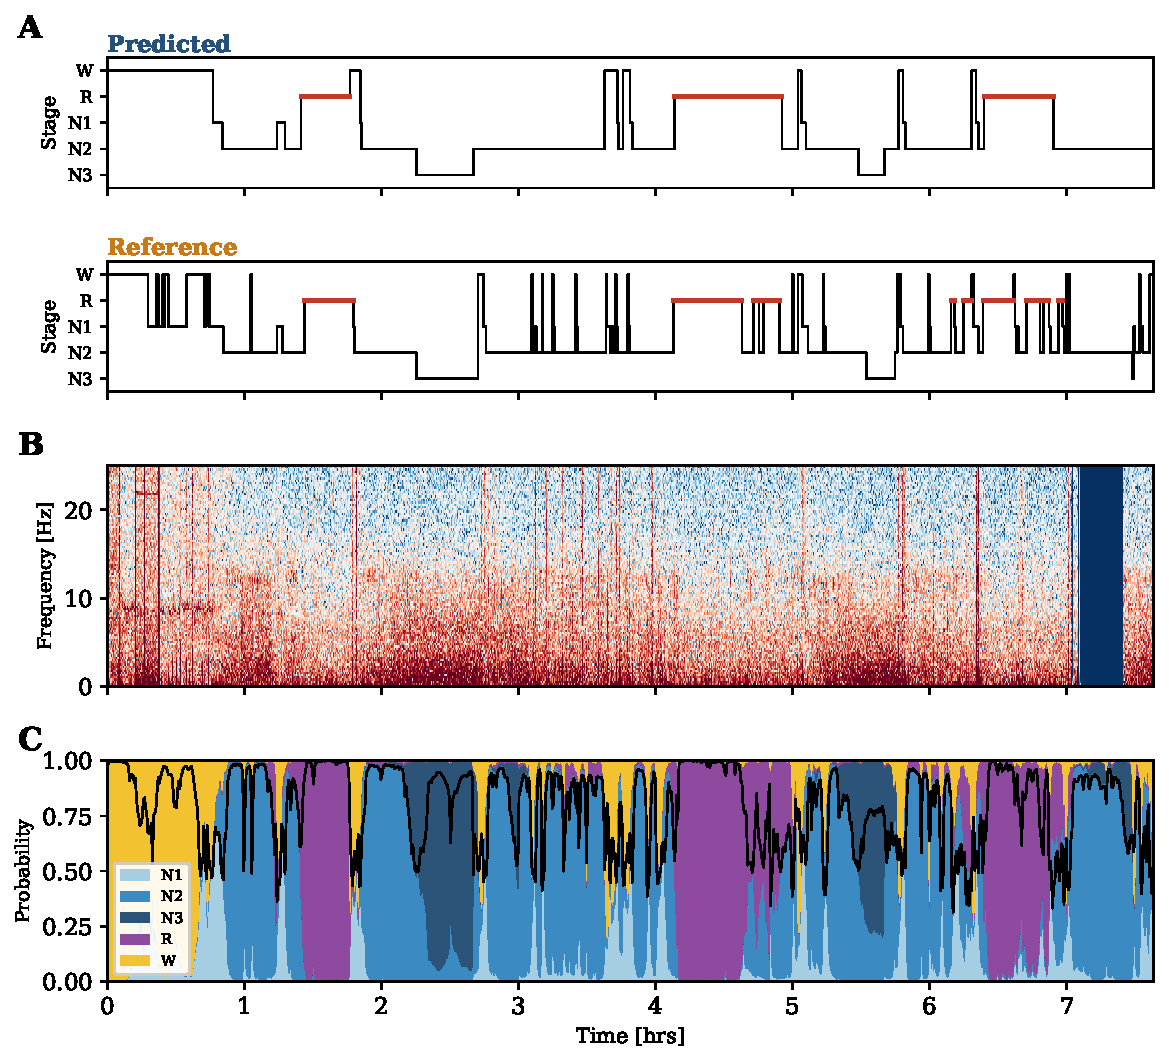
\includegraphics[width=0.86\textwidth]{figures/fig_hypnogram.pdf}
\caption{A representative held-out night (patient SN90, staging accuracy $0.80$).
\textbf{(A)} Predicted and reference hypnograms, REM highlighted. \textbf{(B)} EEG
spectrogram, C4 derivation, $0$--$25$\,Hz. \textbf{(C)} Per-epoch stage-probability
ribbon; the black line is the maximum posterior.}
\label{fig:hypno}
\end{figure*}


\subsection{Per-class Staging Performance}
Table~\ref{tab:perclass} breaks staging down by stage. The pattern is the one this cohort
imposes on every method: N2, Wake, and REM are recovered well, N3 is moderate, and N1 is the
hard stage, because it is transient and rare. The raw convolutional network reaches the highest
N1 F1, which fits its sensitivity to short events, while the proposed model leads on the stable
stages. The row-normalised confusion matrix (Fig.~\ref{fig:confusion}) shows
where the errors land: N1 is absorbed mainly into Wake and N2, and part of N3 is read as N2.
Comparing the neural-only and full rows isolates what the cardiorespiratory stream
contributes to staging, and the answer is narrow: N1 improves by $0.019$ (Wilcoxon
$p=0.11$ on ten fold-means, not significant) and no stage changes significantly
($p \geq 0.15$; REM shifts by $0.01$ in Table~\ref{tab:perclass}, well inside that). That the gain
lands on N1 is consistent with its physiology. It is the transitional stage, the hardest
to score, and the one most often coincident with a respiratory event.

\begin{figure}[t]
\centering

\includegraphics[width=0.82\columnwidth]{figures/fig_confusion.pdf}
\caption{Row-normalised confusion matrix for the proposed model (pooled ten-fold test epochs,
hidden-Markov operating point). Errors concentrate on N1, which is absorbed into Wake and N2.}
\label{fig:confusion}
\end{figure}

\begin{table}[t]
\caption{Per-class staging F1 (Wake, N1, N2, N3, REM), ten-fold patient-independent, at the
hidden-Markov operating point. The neural-only and full rows are means over the same thirty
fold-values. Best per column in \textbf{bold}.}
\label{tab:perclass}
\centering
\setlength{\tabcolsep}{6pt}
\begin{tabular}{lccccc}
\toprule
Model & W\,$\uparrow$ & N1\,$\uparrow$ & N2\,$\uparrow$ & N3\,$\uparrow$ & R\,$\uparrow$ \\
\midrule
Raw multimodal CNN                & 0.74 & \textbf{0.37} & 0.73 & 0.56 & 0.67 \\
MM-Net (neural only)              & \textbf{0.79} & 0.28 & 0.80 & 0.71 & \textbf{0.76} \\
\textbf{MM-Net (neural + cardio)} & 0.79 & 0.30 & \textbf{0.80} & \textbf{0.71} & 0.75 \\
\bottomrule
\end{tabular}
\end{table}

\subsection{Modality-Ablation Grid}
\label{sec:ablate}
This ablation is also our attribution method. Because the model is feature-based and never sees
a raw spectrogram or a raw EEG trace, a gradient heat-map or Grad-CAM would have no
faithful spatial support on the neural side, which is where a staging attribution would be
read; we
therefore attribute each output by \emph{interventional} ablation, deleting a physiological
channel and measuring the change. This is a falsifiable test of what each modality contributes.
The proposed model stages sleep at $\mmAcc$ accuracy ($\kappa$ $\mmK$) and detects respiratory
events at $\mmAuc$ AUC ($\mmAp$ average precision). To test the paper's central claim, that each
modality carries the task its physiology is closest to, we remove each modality in turn and keep the
rest, on the same folds, with three seeds giving thirty fold-values per row
(Table~\ref{tab:ablate}). The separation between streams is clean, but within the
cardiorespiratory stream the pattern is not the one the engineered features gave.

Removing the whole cardiorespiratory stream drops respiratory AUC from $\mmAuc$ to $0.654$,
the largest single effect in this study, and leaves staging untouched ($0.741$, n.s.).
Removing the neural stream does the reverse: staging falls from $\mmAcc$ to $0.680$ while
respiratory detection holds. No neural ablation moves respiratory AUC and no cardiorespiratory
ablation moves staging, so each stream serves the outcome its physiology is closest to.

Within the cardiorespiratory stream, however, only respiratory effort is individually necessary
($-0.038$ AUC, Holm $p=0.018$). Removing SpO$_2$, pulse/HRV, ECG or airflow individually costs
at most $0.005$ AUC and none survives correction; SpO$_2$, which the engineered-feature
configuration was built around, is here among the least necessary channels
($-0.002$, $p=1.00$). The five
individual removals sum to $-0.046$ AUC against $-0.128$ for removing the stream as a whole,
a factor of $2.8$. The learned encoder therefore distributes respiratory information redundantly
across channels: each is individually dispensable because the others overlap it, while the
ensemble is essential. That redundancy is clinically favourable, since
twelve of the ninety-nine recordings are missing at least one cardiorespiratory channel, and it is
physiologically coherent: the effort belts register the paradoxical thoraco-abdominal motion
of an obstructive event as it happens, whereas desaturation is a lagged consequence of it.

\subsection{What the Joint Objective Contributes}
\label{sec:joint}
The ablation grid asks which physiology carries which output. A different question is
whether the two outputs should share a network at all, and nothing so far answers it: a
model that produces two outputs has demonstrated integration, not benefit. The control is a
pair of single-task models, and it has to be matched properly or it measures the wrong
thing. Ours changes one line. The architecture, the ten folds, the three seeds, the
optimiser, the budget and the cardiorespiratory bypass are those of the full model; only the
surviving term of $\mathcal{L}=\mathcal{L}^{\mathrm{stg}}+\lambda\mathcal{L}^{\mathrm{apn}}$
differs, so the staging-only model still builds the cardiorespiratory stream and still feeds
the respiratory head and simply never receives a respiratory gradient. What separates the
rows is the objective and not the network.

Training both tasks together is better than training either alone
(Table~\ref{tab:joint}). Staging rises from $0.733$ to $\mmAcc$ accuracy, in nine folds of
ten (Wilcoxon on the ten fold-means, $p=0.014$), and $\kappa$ from $0.625$ to $\mmK$ on the
same nine. Respiratory AUC rises from $0.774$ to $\mmAuc$ in seven folds of ten ($p=0.049$).
Average precision moves $+0.005$ and does not separate ($p=0.63$), which we report as the
null it is.

Two readings of that are available and only the narrower one is supported. The gains are
small: $0.006$ accuracy against a fold-to-fold SD of $0.019$, and $0.007$ AUC against
$0.038$, so roughly a third and a fifth of the spread the cohort already imposes. What
carries them is consistency instead of size, nine and seven folds of ten moving the same
way, which is what the paired test is reading. The claim we make is therefore that the
second task costs the first nothing and returns a little to it, which is the claim the
architecture needs: a clinician gets the respiratory read-out without trading away staging
accuracy for it. We do not claim multi-task learning as a source of large gains here.

The two diagnostic cells are what make the comparison trustworthy. The respiratory-only
model stages at $0.303$ accuracy and $\kappa$ $0.039$, and the staging-only model detects at
$0.495$ AUC. Both are chance for their untrained head, which confirms that the switch
isolated the loss and did not quietly leave the other objective running.

\begin{table}[t]
\caption{The joint objective against matched single-task models, ten-fold
patient-independent, three seeds. Every row shares the architecture, folds, seeds and
budget; only the surviving loss term differs. $p$ is Wilcoxon on the ten fold-means, the
unit used throughout. The upper cells of each block are the metric that model was trained
for; the lower, in grey, are its untrained head and are chance by construction.}
\label{tab:joint}
\centering
\small
\setlength{\tabcolsep}{5pt}
\begin{tabular}{llccc}
\toprule
Trained on & Metric & Single & Joint & $p$ \\
\midrule
\multirow{2}{*}{Staging only}
 & Accuracy & $0.733$ & $\mathbf{\mmAcc}$ & $\mathbf{0.014}$ \\
 & $\kappa$ & $0.625$ & $\mathbf{\mmK}$   & $\mathbf{0.014}$ \\
\addlinespace[2pt]
\multirow{2}{*}{Respiratory only}
 & AUC & $0.774$ & $\mathbf{\mmAuc}$ & $\mathbf{0.049}$ \\
 & AP  & $0.414$ & $0.419$           & $0.63$ \\
\midrule
\multicolumn{5}{@{}l}{\emph{Untrained heads, reported as the check that the switch worked}}\\[1pt]
Respiratory only & Accuracy & $0.303$ & --- & --- \\
Staging only     & AUC      & $0.495$ & --- & --- \\
\bottomrule
\end{tabular}
\end{table}

\subsection{Recordings With an Incomplete Montage}
Those twelve recordings are scored with the absent channels zero-filled instead of being
excluded, which raises a fair question: does the network read missingness instead of
physiology? It does not appear to. Removing all twelve from the pooled respiratory
evaluation moves AUC from $0.778$ to $0.775$ and moves average precision the other way,
from $0.419$ to $0.439$, so the respiratory result does not rest on them. Predicted
per-patient burden is independent of whether a montage was complete ($p=0.91$), so the
shortcut is not available even in principle.

Staging is lower on those twelve, $0.670$ against $0.743$ ($p=0.017$), and that needs a
control rather than an assurance. The neural-only configuration receives no
cardiorespiratory channel at all and so has nothing zero-filled, yet it shows the same
gap in the same direction, $0.689$ against $0.744$ ($p=0.040$). Most of the difference
therefore belongs to the recordings, which are harder for a model that cannot see the
missing channels either. Stated precisely rather than generously: on those twelve the
full model sits $0.019$ below neural-only, which at $n=12$ is not distinguishable from
noise (Wilcoxon $p=0.18$), so a small cost cannot be excluded, only bounded. On the
eighty-seven complete recordings the two agree to within $0.002$.
Attention and plain concatenation stage and detect alike, so the gain comes from the added
modality, and the fusion mechanism has little effect.

\begin{table*}[t]
\caption{Modality-ablation grid (leave-one-out), ten-fold patient-independent,
three seeds. Each row removes one modality and keeps the rest; cells are means over
thirty fold-values. $p$ is Wilcoxon on the ten fold-means, Holm-corrected across the
nine ablations within each metric and \textbf{bold} where it clears $0.05$; the
floor at this sample size is $0.018$.}
\label{tab:ablate}
\centering
\setlength{\tabcolsep}{14pt}
\begin{tabular}{lcccc}
\toprule
Modality removed & Staging acc\,$\uparrow$ & Holm $p$ & Respiratory AUC\,$\uparrow$ & Holm $p$ \\
\midrule
 none (full model)        & $0.739 \pm 0.020$   & ---                 & $0.782 \pm 0.038$   & --- \\
 EEG (neural)             & $0.680$             & $\mathbf{0.018}$    & $0.774$             & $0.92$ \\
 EOG (ocular)             & $0.731$             & $0.08$              & $0.777$             & $1.00$ \\
 EMG (muscle)             & $0.735$             & $1.00$              & $0.778$             & $1.00$ \\
 SpO$_2$                  & $0.742$             & $1.00$              & $0.780$             & $1.00$ \\
 respiratory effort       & $0.741$             & $1.00$              & $0.744$             & $\mathbf{0.018}$ \\
 pulse / HRV              & $0.741$             & $1.00$              & $0.785$             & $1.00$ \\
 ECG                      & $0.737$             & $1.00$              & $0.777$             & $1.00$ \\
 airflow                  & $0.740$             & $1.00$              & $0.778$             & $1.00$ \\
 all cardiorespiratory    & $0.741$             & $1.00$              & $0.654$             & $\mathbf{0.018}$ \\
\bottomrule
\end{tabular}
\end{table*}

\subsection{Physiological Validity of the Respiratory Read-out}
\label{sec:noflow}
Because the events were scored from airflow, a model that keyed on the airflow channel would
be right for a trivial reason. Removing the airflow features leaves detection essentially
unchanged, at $\noflowAuc$ AUC (Table~\ref{tab:ablate}), within one fold standard deviation of
the full $\mmAuc$. The model therefore does not lean on the labeling signal. It reads above all
the straining of the chest and abdomen (the only channel whose removal costs significantly),
together with the fall in blood oxygen, the beat-to-beat change in the heart, and the
cortical arousal that ends the event, none of which is individually indispensable because the
learned encoder encodes them redundantly. This is the useful regime, because it detects the
bodily consequences of disordered breathing, not a repeat of a measurement a technician
has already made. It is also the physiologically expected one: the effort belts register the
paradoxical thoraco-abdominal motion of an obstructive event while it is happening, whereas
desaturation follows it by several breaths.

\subsection{Respiratory Baselines and Per-event-type Detection}
The respiratory task needs real competitors (Table~\ref{tab:resp}), on the same folds.
The classical baselines read the $14$ engineered cardiorespiratory descriptors; the proposed
model reads the raw signal through its learned encoder, and its own score on the $14$
descriptors is $0.698$ (Table~\ref{tab:repr}), which is the like-for-like comparison. A clinical desaturation rule reaches $0.596$ AUC, logistic
regression $0.582$, and gradient boosting $0.670$; a random classifier scores $0.157$ average
precision, the event prevalence. The proposed model reaches $\mmAuc$ AUC and $\mmAp$ average
precision, above gradient boosting but by a modest margin, so the contribution is the joint
single pass and the physiological attribution above; we do not claim state-of-the-art
detection accuracy. Detection also separates by event type: the model scores $0.748$ AUC on hypopneas (the
mild, dominant $81\%$ of events), $0.898$ on obstructive apneas, and $0.935$ on central apneas.
It is strongest on the most severe events, and the overall AUC is held down by the abundant
hypopneas.

\begin{table}[t]
\caption{Event-level detection, pooled over the ten patient-independent folds
($8{,}400$ scored events over $771$ hours). Within a patient an event is a maximal run of
consecutive epochs, with no gap tolerance, and counts as detected when any epoch inside it
is flagged; a false alarm is a flagged run overlapping no scored epoch, and the rate
denominator is the whole recording, wake included. One flagged run spanning several events
therefore marks each detected while costing at most one false alarm, which is where the
under-counting below comes from. The flagged
fraction is the share of all epochs the threshold marks.}
\label{tab:event}
\centering
\small
\begin{tabular}{cccc}
\toprule
Threshold & Event sens.\,$\uparrow$ & False alarms/h\,$\downarrow$ & Epochs flagged \\
\midrule
$0.2$ & $0.854$ & $3.21$ & $59\%$ \\
$0.3$ & $0.792$ & $3.25$ & $49\%$ \\
$0.4$ & $0.727$ & $3.05$ & $41\%$ \\
$0.5$ & $0.660$ & $2.82$ & $34\%$ \\
$0.6$ & $0.576$ & $2.42$ & $27\%$ \\
$0.7$ & $0.469$ & $1.94$ & $20\%$ \\
\midrule
\multicolumn{4}{@{}l}{\emph{Per-patient agreement with the clinical index}}\\[1pt]
\multicolumn{3}{@{}l}{Aggregated epoch probability (burden)} & $\rho=0.491$ \\
\multicolumn{3}{@{}l}{Counted events per hour} & $\rho=0.148$ \\
\multicolumn{3}{@{}l}{Predicted vs scored event rate} & $4.8$ vs $11.0$ \\
\bottomrule
\end{tabular}
\end{table}

Scoring at the event level instead of the epoch level worsens the picture
(Table~\ref{tab:event}). No threshold is comfortable: the one that finds most events flags
three fifths of the night, and the one that flags least finds under half of them. More
tellingly, the model recovers the wrong \emph{number} of events, and its per-patient event
count agrees with the clinical index far more weakly than its aggregated epoch probability
does ($\rho=0.148$ against $\rho=0.491$). Consecutive events separated by a few epochs merge
into one flagged run, so an epoch-level detector systematically under-counts. This is why we
report a burden, and why event-level scoring is the natural next step instead of a
formality.

Figure~\ref{fig:rocpr} shows the operating characteristics behind these numbers, computed
from the pooled held-out predictions of all ten folds. The precision--recall panel is the
more informative of the two: respiratory events occupy $16\%$ of epochs, and under that
imbalance a ROC curve flatters any detector. Read at fixed sensitivity, the trade-off is
explicit: at $0.80$ sensitivity the model holds $0.59$ specificity and $0.27$ precision,
and pushing sensitivity to $0.90$ costs both, $0.40$ and $0.22$. Either way this is a
research-grade burden estimate, not a scoring-grade detector, and we
describe it as
such. We also note that pooling every fold's epochs into a single curve is not the same
estimator as averaging the ten per-fold scores: pooling weights folds by epoch count and
mixes their score scales, giving a pooled AUC of $0.777$ against the cross-validated
$\mmAuc \pm 0.038$ reported in Table~\ref{tab:resp}. Both are stated so the difference is
visible; at $0.005$ it is an eighth of one fold standard deviation.

\begin{figure}[t]
\centering
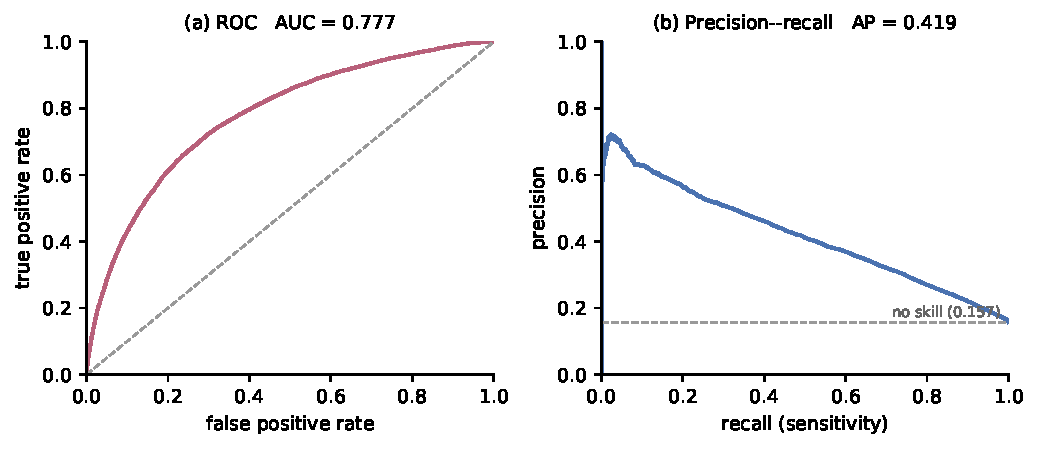
\includegraphics[width=\columnwidth]{figures/fig_roc_pr.pdf}
\caption{Respiratory-event detection, pooled over the ten patient-independent test
folds. \textbf{(a)} Event-level operating characteristic. Each point is a decision
threshold, labelled and sized by the fraction of all epochs it flags.
\textbf{(b)} Precision--recall; the dashed line is the $0.157$ event prevalence, the
no-skill floor.}
\label{fig:rocpr}
\end{figure}

\begin{table}[t]
\caption{Respiratory-event detection, ten-fold patient-independent. \textit{(a)}
Detectors on the same folds; the classical baselines read the $14$ descriptors, MM-Net the
raw signal. Chance average precision is the $0.157$ prevalence. \textit{(b)} AUC by event
type, $96$ annotated patients. Best per column in \textbf{bold}.}
\label{tab:resp}
\centering
\small
\begin{tabular}{lcc}
\toprule
\multicolumn{3}{l}{\textit{(a) Detection method}}\\
\midrule
Method & AUC\,$\uparrow$ & AP\,$\uparrow$ \\
\midrule
Desaturation rule    & 0.596 & 0.214 \\
Logistic regression  & 0.582 & 0.193 \\
Gradient boosting    & 0.670 & 0.290 \\
MM-Net (proposed)    & \textbf{0.782} & \textbf{0.419} \\
\bottomrule
\end{tabular}

\vspace{4pt}
\begin{tabular}{lcc}
\toprule
\multicolumn{3}{l}{\textit{(b) MM-Net AUC by event type}}\\
\midrule
Event type & Positive epochs & AUC\,$\uparrow$ \\
\midrule
Hypopnea    & 11{,}605 & 0.748 \\
Obstructive & 1{,}661  & 0.898 \\
Central     & 831      & \textbf{0.935} \\
\bottomrule
\end{tabular}
\end{table}

\subsection{Clinical Validation against AHI and Severity}
Aggregating the per-epoch respiratory probability into a per-patient burden and correlating it
with the clinical apnea-hypopnea index (AHI) from the metadata gives a significant positive
association (Spearman $\rho=0.491$, $p<0.001$, $n=99$, the twelve recordings with an
incomplete cardiorespiratory montage scored with those channels zero-filled;
Fig.~\ref{fig:ahi}), so the model's output tracks a
clinician's summary measure beyond an epoch-level score. Staging, in turn, degrades as
sleep-disordered breathing worsens: accuracy falls from $0.769$ in patients with a normal AHI to
$0.719$ in the severe group (Table~\ref{tab:severity}). The pathology that motivates the second output also makes the first
harder, which is the clinical reality of this cohort.

The association is real but modest, and it is worth saying why it is
so. Three mechanisms plausibly cap it, and each is a property of the formulation rather
than of the model. First, mean per-epoch probability is a poor estimator of an hourly event
rate: a $30$-second epoch holding one hypopnea and one holding three both contribute a
single positive, so the aggregate compresses exactly the variation the index is built from.
Second, the clinical index is normalised by total sleep time, whereas our burden averages
over every scored epoch including wake, and the two denominators diverge most in the
patients with the most fragmented sleep, which in this cohort is the severe group.
Third, the AHI itself carries substantial night-to-night variability, so a single-night
reference sets a ceiling on any correlation with it. We therefore read $\rho=0.491$ as
evidence that the read-out tracks severity at the group level, without claiming that it
estimates an index.

\begin{figure}[t]
\centering
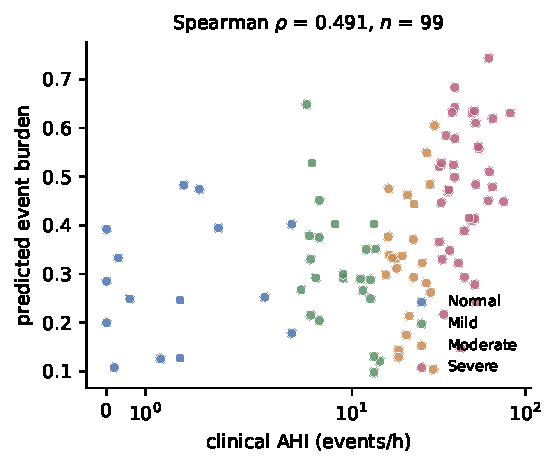
\includegraphics[width=0.86\columnwidth]{figures/fig_ahi.pdf}
\caption{Predicted per-patient event burden (mean respiratory probability) against the clinical
apnea-hypopnea index, coloured by AASM severity band. The positive association (Spearman
$\rho=0.491$, $n=99$) shows the model's output tracks a clinician's summary measure.}
\label{fig:ahi}
\end{figure}

\begin{table}[t]
\caption{Sleep-staging accuracy by sleep-disordered-breathing severity (AASM AHI bands),
ten-fold patient-independent; mean\,$\pm$\,SD across patients ($N=99$). Staging degrades
monotonically as severity rises.}
\label{tab:severity}
\centering
\small
\begin{tabular}{lccc}
\toprule
AHI band & AHI (events/h) & Patients & Staging acc\,$\uparrow$ \\
\midrule
Normal   & $<5$       & 15 & $0.769 \pm 0.049$ \\
Mild     & $5$--$15$  & 23 & $0.747 \pm 0.069$ \\
Moderate & $15$--$30$ & 23 & $0.722 \pm 0.088$ \\
Severe   & $\geq 30$  & 38 & $0.719 \pm 0.100$ \\
\bottomrule
\end{tabular}
\end{table}

\subsection{Permutation Importance: a Second, Independent Attribution}
The ablation grid establishes what the model \emph{needs}: remove a modality, retrain, and
observe which head suffers. A complementary question is what a \emph{trained} model actually
uses. We therefore permute each modality's features across epochs at inference time, so the
channel is still present but no longer aligned to the epoch it describes, and measure the
drop, averaged over three shuffles and the ten fold models.

The two methods can disagree, because a model may need a channel during training yet weight it
lightly afterwards. On staging they do not: permuting the neural features costs $0.284$ staging
accuracy against $0.030$ for the ocular and $0.006$ for the muscle channel, the same ordering
the ablation gives, and the rank correlation between the two attributions is $\rho=0.833$
($p=0.010$).

On the respiratory head the agreement is narrower, and we state it precisely instead of
pooling the two into a single coefficient. Both methods place respiratory effort first by a wide
margin: $0.038$ AUC under retraining, $0.071$ under permutation, in each case well clear of
the runner-up. The remaining four cardiorespiratory channels, however, have retraining effects
that are not distinguishable from zero, so their rank order carries no signal there and the
correlation over the five is correspondingly uninformative ($\rho=0.381$, $p=0.35$).

Permutation separates them where retraining cannot. Each fold records its own baseline
AUC and its AUC after shuffling, so the drop is a within-fold quantity and can be tested
directly. Every channel's drop is distinguishable from zero (one-sample on ten per-fold drops,
Holm across the eight channels): effort $0.071$ ($p<10^{-4}$), airflow $0.027$ ($p=0.0005$),
SpO$_2$ $0.016$ ($p=0.0002$), pulse/HRV $0.012$ ($p=0.004$), and the remainder below $0.006$.
Significance here is not importance. The magnitudes span a factor of $32$, and what the test
establishes is that the \emph{ordering} is real. The ordering is the
result worth having: the three channels the model leans on most, effort, airflow and SpO$_2$,
are exactly the three the AASM definition of a respiratory event is written in, and they are
one to two orders above the cardiac and muscle channels.

The two experiments answer different questions, so the divergence is informative. Retraining without a channel measures whether it is \emph{irreplaceable}, and
the network compensates by re-learning the signal from its correlates; permutation holds the
fitted model still and measures what it \emph{uses}. SpO$_2$ is the clearest case: retraining
without it costs $0.002$ AUC, shuffling it under the fitted model costs $0.016$. A channel can
be heavily used and still be replaceable. The claim the comparison supports is therefore the
one that matters physiologically: two attributions sharing no machinery, one applied to
retrained models and one to fixed ones, independently identify effort as the dominant
respiratory cue.

\subsection{Data Efficiency and the Cohort Ceiling}
\label{sec:curve}
Staging on this corpus saturates near $0.72$--$0.75$ for every model family tried here and
elsewhere. Whether that reflects the architecture or the cohort is testable: retrain the
identical model on a shrinking fraction of the \emph{training patients}, always evaluating on
the full held-out fold (Fig.~\ref{fig:curve}). Subsampling is by patient,
because epochs within a patient are heavily correlated.

The two heads answer differently. Staging accuracy rises $0.701 \rightarrow 0.721 \rightarrow
0.726 \rightarrow 0.735$ as training patients go from $20$ to $79$, with marginal gains of
$+0.020$, $+0.005$ and $+0.009$, all under half a fold standard deviation and flattening.
Respiratory AUC over the same range rises $0.732 \rightarrow 0.750 \rightarrow 0.752
\rightarrow 0.785$, and its \emph{largest} increment is the final one, $+0.033$, close to a
full fold standard deviation, and steeper than any earlier step. This curve is a single seed
on a fixed held-out set, so its endpoint differs slightly from the three-seed headline figures
($\mmAcc$ and $\mmAuc$); the shape is what this curve is here to show. Staging has stopped
responding to added patients at this sample size; respiratory detection has not, and is still
accelerating. We draw the
narrower conclusion the data support: over the range we can test, more patients of this kind
would improve breathing detection and would not appreciably improve staging. That is a
statement about the returns to cohort size for these methods. It is not a measurement of an
irreducible error rate, which fewer than a hundred patients and a finite set of architectures
cannot establish. The final model also exceeds
the feature-only configuration at the full training-set size, so its advantage is not an
artefact of the full sample.

\begin{figure}[t]
\centering
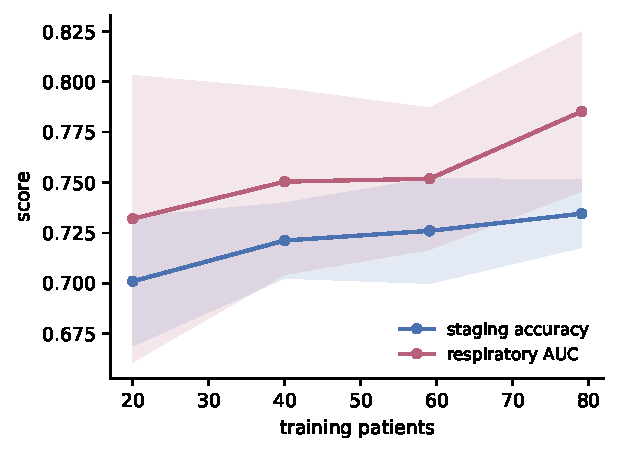
\includegraphics[width=0.86\columnwidth]{figures/fig_learning_curve.pdf}
\caption{Learning curve over training-patient fraction, ten-fold patient-independent, error
bars one standard deviation across folds. Staging (blue) flattens by $57$ patients; respiratory
detection is still climbing at $76$. Bands are $\pm$ one standard deviation
across folds.}
\label{fig:curve}
\end{figure}

\subsection{Healthy-Trained Models Applied to the Injured Brain}
\label{sec:domaingap}
Table~\ref{tab:bench} retrains published architectures \emph{on} iSLEEPS. A different and
harder question is what happens when a model built for healthy sleep is applied to this cohort
as published. The three architectures are our own: a four-channel CNN, the same
CNN with a BiLSTM over epochs, and StagingSeqNet, a deeper convolutional-recurrent stager we
built for this comparison. Naming them matters only in that none is a weak straw man; each
reaches $0.81$ to $0.87$ on the healthy corpus it was trained on. We trained them on the
Sleep-EDF Cassette subset and applied each to all
$99$ iSLEEPS patients zero-shot, with no adaptation of any kind. This is the middle block of
Table~\ref{tab:bench}, set against the same architectures retrained on this cohort.

The result is not a degradation but a collapse. All three stage healthy sleep competently,
$0.806$ to $0.855$ accuracy and $\kappa$ $0.73$ to $0.81$; on stroke the same checkpoints reach
$0.306$ to $0.312$ with $\kappa$ $0.09$ to $0.13$, which is close to chance for a five-class
problem with this prior. The failure mode is more informative than the headline. Wake takes
$62$ to $79\%$ of predicted stroke epochs against a true $26.7\%$, while N2 falls to between
$1$ and $5\%$ of predictions on the stage that is $42.3\%$ of the data, and N2 recall on the
worst of the three is $0.015$. These models do not lose accuracy
gracefully; they stop recognising sleep architecture at all.

The control is what makes this interpretable. A healthy-trained stager scoring $0.31$
on iSLEEPS is evidence of a cohort effect only if the same checkpoint, through the same
preprocessing, scores properly on healthy sleep; otherwise a broken input pipeline and a
genuine domain gap produce identical numbers. Run through our pipeline on held-out Sleep-EDF
recordings, the strongest checkpoint holds at $0.8682$ ($0.8667 \pm 0.0415$ per recording), so
the pipeline is correct and the collapse belongs to the cohort.

Two bounds, reported together. Sleep-EDF is recorded on Fpz-Cz and Pz-Oz where iSLEEPS
uses C4:M1 and O2:M1, so part of this gap is montage shift, not pathology, and quoting
the zero-shot number alone would overstate the case. Deep models trained \emph{on} iSLEEPS with
the matched montage reach $0.61$--$0.69$ (upper block), which puts the cost of
pathology alone at roughly $0.19$ against healthy-sleep performance; healthy-trained and
zero-shot, with the montage shift included, the cost is $0.56$. The claim is bounded by those two figures together.

The same argument run in reverse. Every figure above concerns other
architectures, which leaves the obvious question unanswered: whether $\mmAcc$ is low
because the cohort is hard or because the proposed model is weak. So we cross-validated it
on healthy sleep, ten-fold and subject-independent over the $21$ Sleep-EDF subjects, using the
neural branch alone since that corpus carries none of the cardiorespiratory channels we read. It reaches
$0.856 \pm 0.027$ accuracy with $\kappa$ $0.800$ (final row of Table~\ref{tab:bench}).
That places it among the healthy-sleep stagers in the middle block,
against $0.741$ for the identical architecture on stroke. The $0.115$ difference is what
the cohort costs a model that is demonstrably capable of more, which is a stronger
statement than any comparison against other people's architectures can make.

The cohort does not cost every architecture equally. Because the three reimplemented
models carry a healthy-sleep score produced by the same code under the same protocol, the
table supports a comparison it could not before: not merely where each model lands, but how
much it loses in the crossing. TinySleepNet falls $0.148$ from healthy sleep to stroke
($0.824 \to 0.676$), SleepTransformer $0.140$ ($0.823 \to 0.683$) and U-Time $0.145$
($0.791 \to 0.646$), against $0.115$ for the proposed model ($0.856 \to 0.741$). It is therefore not simply higher at both ends; it
degrades least. We report this as an observation. Four paired differences
will not support a significance test, and the comparison is between systems rather than a controlled ablation, since the proposed rows read engineered features and a frozen embedding
over four derivations while the three reimplemented baselines read a single raw channel. The
direction is nonetheless the one the rest of the paper predicts: a representation that
encodes sleep physiology explicitly survives a disordered cortex better than one a network
must discover for itself from fewer than a hundred patients.

Folds are split by subject, not by recording, because Sleep-EDF Cassette records
each subject on two nights; splitting on filenames would place the same person on both
sides of a fold.



\subsection{Stream Representations}
\label{sec:repr}
The architecture makes two representation choices (engineered features plus a frozen
self-supervised embedding on the neural side, a learned convolutional encoder over the raw
signal on the cardiorespiratory side), and both were selected by experiment, not
assumed. Each family below holds every other hyperparameter fixed and varies one thing, over
the same three seeds and ten patient-independent folds, with Holm correction within the
family and every test on the ten fold-means.

The cardiorespiratory features are the bottleneck, and part of the gap needs no new
information. Each block of Table~\ref{tab:repr} holds the other stream at its baseline, so no single
row there is the full model, and the two baselines differ: the cardiorespiratory block runs
the $188$ neural descriptors without the pretrained embedding, while the neural block runs the
$14$ engineered cardiorespiratory descriptors. That is why the two blocks report different
respiratory AUC for what both call an engineered-feature reference ($0.698$ against $0.685$),
and why the adopted cardiorespiratory row reads $0.740$ staging accuracy against the headline
$\mmAcc$, which adds the pretrained embedding on top of it. The upper block replaces the $14$ engineered cardiorespiratory features
with progressively richer representations of the same underlying signal. Every step is
significant, and the ordering is instructive. A \emph{random} nonlinear expansion of the same
$14$ numbers recovers $0.018$ AUC: that gain needs no new measurement at all, only more
capacity to read what was already computed, which says the summary features leave nonlinear
structure unextracted. A random linear projection of the raw waveform adds a further $0.016$,
so part of what the features discard is recoverable without learning anything. The learned
convolutional encoder reaches $0.782$, $0.084$ above the engineered features.

What this establishes is that the representation of the cardiorespiratory stream, and not the detector on top of it, is what limited the respiratory read-out. We therefore claim the
change of representation itself, and make no claim for the encoder that implements it.

On the neural side a pretrained encoder does not replace expert features, but does
add to them. The lower block of Table~\ref{tab:repr} varies the neural representation with the
cardiorespiratory stream held at the engineered features. Used alone, the frozen encoder is
significantly \emph{worse} than the $188$ features ($-0.029$, Holm $p=0.008$): pretraining on
healthy scalp EEG does not by itself substitute for physiology chosen for this task.
Concatenated with the features it adds $+0.008$ accuracy (Holm $p=0.006$), and a second
pretrained encoder on top of the first adds nothing further ($-0.004$, $p=0.56$).

The reading we take is narrow, because it is what the numbers support: expert physiology and
self-supervised pretraining encode partly different information, so their union beats either
alone; but the complementarity saturates after one pretrained encoder, so this is not a
general argument for stacking foundation models.

\begin{table*}[t]
\caption{What each stream should be represented as. One factor varies per block,
everything else held fixed; cells are mean $\pm$ SD over thirty fold-values. $\Delta$ and
Holm $p$ are against each block's engineered-feature baseline, the latter on the ten
fold-means. ``adopted'' marks the choice carried into the final model.}
\label{tab:repr}
\centering
\begin{tabular*}{\textwidth}{@{\extracolsep{\fill}} l l c c c c @{}}
\toprule
Representation & Variant & Resp.\ AUC\,$\uparrow$ & Staging acc\,$\uparrow$ & $\Delta$ & Holm $p$ \\
\midrule
\multirow{4}{*}{\emph{Cardiorespiratory}}
 & $14$ engineered features               & $0.698 \pm 0.051$ & $0.736 \pm 0.014$ & ---      & ---      \\
 & random nonlinear expansion of the $14$ & $0.715 \pm 0.047$ & $0.737 \pm 0.018$ & $+0.018$ & $0.012$   \\
 & random linear projection of raw signal & $0.731 \pm 0.044$ & $0.735 \pm 0.021$ & $+0.034$ & $0.012$   \\
 & learned CNN, $0.155$\,M (adopted)      & $\mathbf{0.782 \pm 0.040}$ & $0.740 \pm 0.019$ & $+0.084$ & $\mathbf{0.006}$ \\
\midrule
\multirow{4}{*}{\emph{Neural}}
 & $188$ engineered features            & $0.685 \pm 0.041$ & $0.741 \pm 0.016$ & ---      & ---      \\
 & frozen pretrained encoder alone      & $0.681 \pm 0.033$ & $0.712 \pm 0.033$ & $-0.029$ & $0.008$   \\
 & features $+$ pretrained (adopted)    & $0.690 \pm 0.037$ & $\mathbf{0.749 \pm 0.018}$ & $+0.008$ & $\mathbf{0.006}$ \\
 & features $+$ two pretrained encoders & $0.684 \pm 0.043$ & $0.745 \pm 0.018$ & $+0.004$ & $0.23$   \\
\bottomrule
\end{tabular*}
\end{table*}

\subsection{The Two Loss Constants}
\label{sec:losssens}
Two constants in Section~\ref{sec:method} were fixed by argument instead of by experiment:
the task balance $\lambda=1$ and the positive weight $\pi=n_-/n_+$, which is $5.35$ on this
corpus. Equal coefficients do not make equal influence, since the two terms differ in scale
and curvature, so $\lambda=1$ is a claim about arithmetic and not about balance. We therefore
swept each with everything else at the published setting, three seeds by ten folds per value,
and read both heads at every point, because the failure worth finding is not a lower number
on one head but a trade between them.

There is no trade, and there is very little effect. Across $\lambda$ from $0.25$ to $4$
staging accuracy spans $0.003$ and respiratory AUC $0.018$, and across $\pi$ from $1$ to $11$
they span $0.003$ and $0.007$; the fold-to-fold standard deviations are $0.019$ and $0.038$.
Both heads also peak at the same $\lambda$, which is the specific thing a compromise would
have ruled out: if $\lambda=1$ were balancing one task against the other, the two curves
would peak on opposite sides of it.

Neither published value is quite the best of those tested. Staging is highest at $\lambda=2$
($0.7403$) and at $\pi=11$ ($0.7422$), and respiratory AUC at $\lambda=2$ ($0.7840$) and
$\pi=8$ ($0.7846$). Every one of those margins is under a fifth of a fold standard deviation,
so we have not found better settings, only confirmed that the objective is insensitive to
both constants over the range a reader would ask about. That insensitivity is the result:
fixing them by fiat costs nothing measurable here.

\subsection{Calibration and Selective Prediction}
A clinical reader needs to know not only how often the model is right but whether it knows when
it is likely to be wrong. Two measurements answer that, both computed on held-out epochs with
the raw posteriors before HMM smoothing.

The model is \emph{overconfident}: expected calibration error, over ten equal-width confidence
bins weighted by occupancy and ignoring bins holding fewer than fifty epochs, is $0.076$, and
the gap runs one
way in every bin: epochs it scores above $0.9$ are correct $88\%$ of the time.
Stated confidences should therefore be read as ordered, not as probabilities, which is the
displacement Section~\ref{sec:method} derives arriving in the measurement.

Ranking, however, is what abstention needs. Applying split-conformal prediction with the
fold's validation patients as the calibration set gives empirical coverage that tracks the
target closely ($0.894$ at a $0.90$ target, $0.943$ at $0.95$). At $\alpha=0.10$ the model
returns a single stage for $45.8\%$ of epochs and is correct on $86.9\%$ of those, against
$59.1\%$ on the epochs where it returns a larger set. The abstention is therefore selecting the
genuinely hard epochs, and it concentrates where a scorer would
expect: N1 receives a singleton set only $19\%$ of the time, the lowest of any stage and the
one human scorers agree on least.

Two caveats attach to the coverage figures rather than to the abstention behaviour. The
calibration patients are the same patients that stopped training, so their labels have already
influenced which checkpoint was kept and they are not the independent calibration sample
split-conformal theory assumes; the coverage we report is therefore empirical and carries no
guarantee. And epochs within a night are strongly dependent, so the exchangeable unit is
closer to the patient than to the epoch, which makes these marginal rates across pooled
epochs and not coverage for a new patient or within any one stage. A calibration split
disjoint from early stopping would settle both, and we did not run one.

\subsection{External Validation on Two Independent Corpora}
\label{sec:external}
Ten-fold cross-validation is patient-independent but remains within one corpus, one centre
and one acquisition protocol. We therefore trained a single model on all $99$ iSLEEPS
patients and evaluated it, unchanged, on two public corpora with no dataset-specific
tuning: no fine-tuning, no threshold search, no re-fitted model or decision threshold (per-recording feature standardisation is applied, as in training), and hidden-Markov
transitions estimated from iSLEEPS alone (Table~\ref{tab:ext}).

The two corpora test different things. \textbf{Sleep-EDF}~\cite{kemp2000sleepedf}
is healthy sleep recorded on a frontal montage (Fpz-Cz, Pz-Oz). Its Cassette recordings carry
an oronasal airflow trace at $1$\,Hz but no ECG, effort belts or oximetry, and no scored
respiratory events, so six of our seven cardiorespiratory inputs are absent and the
respiratory head cannot be scored there; it tests the staging head across both a cohort shift
and a montage shift.
\textbf{ISRUC-Sleep}~\cite{khalighi2016isruc} is a sleep-disorders cohort recorded on the
same central and occipital derivations we use (C4, C3, O2, O1 against the contralateral
mastoid), with SpO$_2$, airflow, effort and ECG, and with obstructive, central and mixed
apneas and hypopneas scored, so it tests the staging head \emph{without} a montage
confound and provides the only external test of the respiratory head. Because Sleep-EDF
carries almost none of those channels, that branch is fed zeros there. Zeroing an input the
network trained on is a train/test mismatch, not an ablation, so we also trained a
model with the branch zeroed throughout: it reaches $0.774$ accuracy against the $0.794$
reported. The two are separate procedures and neither bounds the other, so we report both
and rest nothing on the higher one. The mismatched run could be gaining from batch-normalisation statistics that never
saw zeros, in which case $0.774$ is the more defensible number, and a reader who prefers it
loses nothing in our argument: both sit above the in-domain $\mmAcc$. Both corpora
also differ from iSLEEPS in montage, so both transfer figures are lower bounds and not
clean estimates. ISRUC records each
subject twice; respiratory-event prevalence is $10.1\%$ on the first night and $2.4\%$ on
the second, so we report the two separately instead of pooling a difference that has
nothing to do with the model.

The respiratory read-out transfers. On ISRUC night one the model reaches
$0.780$ AUC, and it does so handicapped, because ISRUC provides no pulse channel and no
separate effort trace, leaving two of the seven cardiorespiratory inputs zero-filled. A
detector that had latched onto one centre's equipment would not survive that; this one does.
The comparison needs its estimators matched to mean anything, and we state them instead of
placing the two numbers side by side. The external figure is pooled over all epochs of the
night, because per-recording AUC is unusable on this corpus: event prevalence ranges from
$0\%$ to $22\%$ across the sixteen recordings, and a night with a handful of positive epochs
returns an estimate whose sampling variance swamps any difference between models, while a
night with none leaves AUC undefined. The in-domain headline $\mmAuc$ is a ten-fold mean.
Pooled in-domain, the like-for-like quantity, is $0.778$. The external result therefore
sits within $0.003$ of the in-domain one on either estimator, and nothing in the claim rests
on which is chosen. Night two falls to $0.723$. Its event prevalence is much lower ($2.4\%$
against $10.1\%$), which does not by itself depress AUC, since ranking is insensitive to the
mix; what the scarcity of positives does is widen the uncertainty on that night's estimate,
so we read the two nights as one imprecise result and not as a trend.

Staging moves in opposite directions on the two corpora, for reasons the data
identify. On Sleep-EDF the model \emph{gains} $0.084$ of $\kappa$ over its in-domain
score. A representation that had memorised corpus-specific artefacts would degrade out of
corpus, so the straightforward reading is that the features are physiological and that the
ceiling reported throughout this paper is a property of \emph{stroke sleep} instead of
the model. The learning curve reaches the same conclusion (Section~\ref{sec:curve}) by a
different route. On ISRUC staging falls by $0.090$ accuracy, and the class mix explains
much of it: ISRUC carries $15.6\%$ N1 against iSLEEPS' $10.2\%$ and Sleep-EDF's $6.6\%$,
and N1 is the weakest stage in every cohort we have measured (recall $0.168$ on ISRUC,
$0.294$ on Sleep-EDF, and the lowest per-class F1 in-domain).

A montage explanation the data now rule out. An earlier version of this
work observed N3 recall of $0.554$ on Sleep-EDF with $44\%$ of N3 epochs read as N2, and
attributed it to slow-wave activity being frontally dominant while the model reads central
and occipital derivations. That account made a prediction: N3 should recover on ISRUC,
which uses our derivations exactly. Under the final model the prediction fails, and it
fails in the direction that rules the explanation out. N3 recall is $0.841$ on Sleep-EDF,
the mismatched frontal montage, with $12.7\%$ of N3 read as N2, and $0.630$ on ISRUC, the
matching one, with $34.8\%$. Electrode position is therefore not what governs N3 transfer
here. The only component that changed between the two models is the neural representation
(Section~\ref{sec:repr}), which points instead at how the cortex is encoded, though with
one external pass per corpus and eight ISRUC subjects we can identify the effect without
attributing it confidently. The prediction stays on the record, and it was wrong.

Two limits keep this in proportion. Accuracy across cohorts with different class balance is
not directly comparable, which is why $\kappa$ is reported alongside. And ISRUC contributes
only eight subjects. Per-recording accuracy spans $0.458$--$0.748$, so the ISRUC
figures in Table~\ref{tab:ext} are quoted to three decimals for consistency with the rest of
the paper and should be read to two; per-recording
respiratory AUC spans $0.515$--$0.848$, with the widest uncertainty on the nights carrying
fewest scored events.

\begin{table}[t]
\caption{External validation, zero-shot: one model trained on all $99$ iSLEEPS
patients, no dataset-specific tuning. In-domain figures are ten-fold means. Sleep-EDF carries
no scored respiratory events and almost none of our cardiorespiratory channels, so the
respiratory head is unscored there; the two ISRUC nights
differ in event prevalence and are reported separately.}
\label{tab:ext}
\centering
\setlength{\tabcolsep}{4pt}
\resizebox{\columnwidth}{!}{%
\begin{tabular}{llcccc}
\toprule
Corpus & Cohort & Rec. & Acc\,$\uparrow$ & $\kappa$\,$\uparrow$ & Resp.\ AUC\,$\uparrow$ \\
\midrule
iSLEEPS (in-domain)   & stroke        & 99 & $\mmAcc$ & $\mmK$ & $\mmAuc$ \\
\midrule
Sleep-EDF             & healthy       & 40 & $\mathbf{0.794}$ & $\mathbf{0.718}$ & --- \\
ISRUC, night 1        & sleep-disord. &  8 & $0.649$ & $0.536$ & $\mathbf{0.780}$ \\
ISRUC, night 2        & sleep-disord. &  8 & $0.575$ & $0.426$ & $0.723$ \\
\bottomrule
\end{tabular}}
\end{table}

\subsection{Model Complexity and Capability}
Table~\ref{tab:cost} sets the proposed model beside representative alternatives on size and
capability. At $2.76$\,M trainable parameters the model is an order of magnitude
smaller than DeepSleepNet ($\sim$$21$\,M) and the corpus's own CNN-ResNet18 ($\sim$$11$\,M),
and comparable to SleepTransformer, so size is not where it wins. It delivers both a
competitive stage and a respiratory read-out from one pass over the recording, and none of
the staging-only models, at any size, can supply the second output.

\begin{table}[t]
\caption{Model size and clinical capability. The proposed model is mid-sized and is the only
one that produces both a stage and a respiratory-event label at competitive staging accuracy;
the raw multimodal CNN produces both but stages at $0.654$.}
\label{tab:cost}
\centering
\setlength{\tabcolsep}{4pt}
\begin{tabular}{lccc}
\toprule
Model & Input & Params\,$\downarrow$ & Outputs \\
\midrule
CNN-ResNet18~\cite{bose2026gap}           & 1\,EEG      & $\sim$11\,M & stage \\
DeepSleepNet~\cite{supratak2017deepsleepnet} & 1\,EEG   & $\sim$21\,M & stage \\
Raw multimodal CNN                        & 14\,ch      & 0.95\,M     & stage + apnea \\
\textbf{MM-Net (proposed)}                & 7\,ch feat $+$ raw & \textbf{2.76\,M} & \textbf{stage + apnea} \\
\bottomrule
\end{tabular}
\end{table}

%=====================================================================
% =========================================================================
% REVISION STATUS, 8 September 2026 -- REMOVE BEFORE SUBMISSION
%
% The model changed. Headline macros (mmAcc, mmMf, mmK, mmAuc, mmAp) now carry
% the final configuration's values, re-run over three seeds and ten folds.
%
% Anything wrapped in \stale{} is still showing numbers from the previous
% feature-only model. Each must be regenerated or removed. Red is a to-do list.
%
% Regenerable on the 5080 from results/revision/runs/final/predictions_seed42.npz:
%   confusion matrix, per-class F1, AHI scatter, severity table,
%   operating characteristics, per-event-type AUC
% Needs its own re-run:
%   modality ablation grid (card_drop must be remapped to raw channel layout),
%   learning curve
% CANNOT be run on the 5080 -- data/isruc_mm and data/sleep_edf_mm absent:
%   external validation. See foundation/EXTERNAL_VALIDATION_INSTRUCTIONS.md
% =========================================================================

\section{Discussion}
The result is a single model that reads the whole sleeping body and speaks to two clinical
questions at once, in the population where both matter. The learned per-epoch embedding separates cleanly by sleep stage while the
respiratory structure stays diffuse, mirroring the strong staging and the modest
respiratory AUC.

 Staging accuracy on this cohort saturates
below $0.75$ for every model family we evaluated, and the proposed model reaches $\mmAcc$ while
adding a respiratory capability the staging models lack. The respiratory
read-out does not depend on the labeling channel: it survives deletion of the airflow channel and
rests on respiratory effort, desaturation, and arousal, the same signs a physician reads at the
bedside.

The $\mmAcc$ staging figure should be judged on this cohort, where healthy-sleep accuracy does not transfer. Deep
architectures developed on healthy sleepers collapse here: DeepSleepNet reaches $0.615$,
CNN-ResNet18 $0.617$, and a network pretrained on the healthy Sleep-EDF corpus and applied to
this cohort $0.623$, each roughly fifteen to twenty points below its healthy accuracy of about
$0.85$. The injured brain distorts the very micro-events, spindles, slow waves, and atonia, that
those models learned to read. What holds up is physiologically grounded modeling on engineered
features, at $0.72$ to $0.75$, which matches the published baseline on this corpus. The lesson is
that healthy-sleep deep learning fails on the injured brain, and this cohort requires
cohort-specific, physiologically grounded, multimodal modeling.

The study also draws a clean physiological line. The cortical channels carry sleep staging, and
the cardiorespiratory channels carry breathing, and the model places each where it belongs
instead of blurring them. That the neural and multimodal variants stage alike is the expected
outcome: the second modality adds a new capability while leaving staging unchanged. We view this separation as a strength for
clinical use, because a reader can trust that the respiratory output reflects breathing and the
staging output reflects the brain.

Separating the modalities is not the same as separating the tasks, and the two questions
come apart. Section~\ref{sec:joint} trains each task alone and finds the joint model ahead
of both, slightly and consistently. So the physiology divides while the objective does not,
which is the arrangement a shared temporal decoder would predict: the streams carry
different information, and the recurrent state that reads them benefits from being asked two
questions about the same ten minutes of sleep.

\subsection{Limitations}
\label{sec:limitations}
The system is offline, and mildly transductive. Two properties follow from
the design and neither is visible in the numbers. Staging uses whole-night Viterbi decoding,
so no epoch can be scored until the recording ends, which rules out the real-time use a
bedside monitor would need. And features are standardised per patient, which at test time uses
that night's own statistics; the model never sees another patient's labels, so this is not
label leakage, but it is a transductive step and a strictly causal deployment would need
running or population statistics instead. We have measured what that substitution costs,
and within the resolution of these folds it costs nothing. Repeating the ten folds with
the standardisation statistics pooled over each fold's training patients and applied
unchanged to the held-out ones moves accuracy by $+0.003$, $\kappa$ by $+0.004$, and
respiratory AUC by $-0.000$, none of which is distinguishable from zero when paired
across folds (accuracy $p=0.28$, AUC $p=1.00$). The per-recording statistics are a
convenience, and the transductive step is not what the numbers rest
on. The whole-night decoding is the real obstacle to bedside use, and it is untouched by
this.

A prediction of ours that failed. The montage account of N3 transfer described in
Section~\ref{sec:external} does not survive retesting under the final model, and we report
it as falsified instead of removing it. Two cautions follow for every other per-class
figure in that section: each rests on a single external pass with no fold structure, so
none carries an interval, and ISRUC contributes eight subjects, at which size a per-class
rate is an estimate with a width we cannot quote. Per-class transfer should be read as
direction, not magnitude.

The evidence comes from a single center and $99$ patients. Section~\ref{sec:external} shows both heads
transfer to independent corpora without tuning, but neither external corpus is a stroke
cohort, so every stroke-specific claim rests on iSLEEPS alone; multi-center validation on
a second stroke cohort is required before clinical use, and no such public corpus
currently exists. The external respiratory result rests on eight subjects, two of whose
seven cardiorespiratory inputs were unavailable, so it establishes that the read-out
transfers, not how well. Respiratory detection, at $\mmAuc$ AUC, is a useful signal but not yet a
screening-grade one, and it is scored per epoch. At
event level it detects $66\%$ of events at $2.8$ false alarms per hour and under-counts
the event rate by more than half, $4.8$ against $11.0$ per hour, so it cannot substitute
for a scored index. The
staging head is also overconfident (expected calibration error $0.076$), so its
posteriors should be used for ranking and abstention. Staging does not improve on the
published baseline for this corpus, and while every architecture we ran saturates in the same
narrow band, we have not established that the band is a limit rather than the reach of the
methods and the sample size we had. Finally, the model is feature-based: it inherits the assumptions of the engineered
representations and is only partly an end-to-end raw-signal learner, since the neural stream reads
engineered descriptors and a frozen embedding while the cardiorespiratory stream is trained on
the raw signal, a deliberate trade for data
efficiency on a small cohort.

\subsection{Future Work}
Two directions follow naturally. Event-level metrics, such as sensitivity per event and false
alarms per hour, would sit beside the epoch-level AUC and speak more directly to a sleep
technician, and finer modeling of the breathing waveforms is likely to raise the respiratory
number further. Linking the multimodal representation to stroke severity and recovery is the
larger opportunity, and one the cardiorespiratory signal is well placed to serve.

%=====================================================================
\section{Conclusion}
We built a model that reads the neural and cardiorespiratory channels of a stroke patient's
polysomnogram and, from one pass,
stages their sleep and detects their respiratory events. Deep networks built for healthy sleep
collapse to $0.61$--$0.72$ accuracy on this cohort, and its $\mmAcc$ sits at the top of the
band every model family we ran reaches here. The contribution is the second output, a respiratory
read-out at $\mmAuc$ AUC that survives removal of the airflow channel, showing it reads the
underlying physiology. Reading the whole recording lets one model report on breathing as well
as on sleep, in the population where breathing matters most. Code and features are released.

%=====================================================================
\appendices
\section{The $188$ Neural Descriptors}
\label{app:features}
Each $30$-second epoch is $3000$ samples at $100$\,Hz, and every descriptor below is
computed on one epoch alone. Nothing is smoothed across epochs, because the
cross-epoch context the model needs is supplied by the recurrent decoder rather
than by the features. Twenty-three descriptors are computed on each of the seven
neural channels, C4:M1, C3:M2, O2:M1, O1:M2, E1:M2, E2:M2 and the chin EMG, which
gives $161$; a further $27$ event descriptors are applied only to the channels whose
physiology defines them, giving $188$ in total.

The per-channel set begins with the spectrum, a Welch estimate over $256$-sample
segments overlapping by $128$. From it we take absolute and relative power in the
five bands of Section~\ref{sec:features}, the logarithm of total power, spectral
entropy on the normalised spectrum, the $95\%$ spectral-edge frequency and the mean
frequency. Six time-domain statistics follow, namely standard deviation,
peak-to-peak, root mean square, skewness, kurtosis and zero-crossing rate, and to
these are added the three Hjorth descriptors, activity, mobility and complexity,
computed from the first and second differences~\cite{hjorth1970eeg}.

The event descriptors follow the graphoelements a scorer reads, and every band-pass
among them is a fourth-order Butterworth applied forwards and backwards so that
phase is preserved. Spindles contribute three descriptors per EEG channel: the
channel is filtered to $11$--$16$\,Hz, its analytic envelope is taken by Hilbert
transform, and the threshold is set at the $90$th percentile of that envelope within
the epoch, so that it tracks the amplitude of the epoch itself instead of a fixed
microvolt level; density counts upward crossings of that threshold, and the mean and
standard deviation of the envelope complete the three. Slow waves contribute two per
EEG channel, the peak-to-peak and the mean absolute amplitude of the $0.5$--$4$\,Hz
band, with no duration or morphology criterion imposed, so that they summarise
slow-wave amplitude and do not detect discrete waves. Each EOG channel contributes
the log mean squared first difference and the $95$th percentile of its absolute
value, which separate the fast deflections of REM from slow drift, and the chin EMG
contributes log root-mean-square, the $90$th percentile of the absolute signal, and
the log variance of the first difference, which together track tonic level and its
loss in REM.

No epoch and no channel is rejected, and no amplitude threshold is applied, so a
corrupted channel reaches the model. The modality ablations of
Section~\ref{sec:ablate} show the streams carry enough redundancy to absorb one, and
any rejection rule would have to be tuned on this cohort. Non-finite values, which
arise only from a flat channel, are set to zero. Each descriptor is finally
standardised against the mean and standard deviation of its own recording, the
transductive step Section~\ref{sec:limitations} returns to, and nothing is
aggregated across epochs.

%=====================================================================
\section*{Data and Code Availability}
The iSLEEPS corpus is publicly available (Zenodo, DOI 10.5281/zenodo.14873844; and the
india-data.org portal) as described by Maiti \textit{et al.}~\cite{maiti2026isleeps}. Our
code, engineered features, and reproduction notebook are released at
\url{https://github.com/wshuv-o/isleeps-sleep-staging}.

\section*{Ethics}
The iSLEEPS data collection was approved by the NIMHANS Institutional Ethics Committee
(No.\ NIMHANS/34th IEC (BS\&NS DIV.)/2022, dated 05.02.2022)~\cite{maiti2026isleeps}. This work
is a secondary analysis of the de-identified public release and required no additional
enrollment.

\section*{Funding}
The authors received no specific funding for this work.

%=====================================================================
\section*{Acknowledgment}
The authors thank the iSLEEPS investigators for releasing the corpus.

\bibliographystyle{IEEEtran}
\bibliography{references}

%=====================================================================
%  AUTHOR BIOGRAPHIES
%

\begin{IEEEbiography}[{
\includegraphics[width=1in,height=1.25in,clip,keepaspectratio]{bio_suva.jpg}}]{MD WAHIDUZZAMAN SUVA}
received the B.Sc. degree in computer science and engineering from American
International University-Bangladesh (AIUB), Dhaka, Bangladesh, in 2025, where he is
currently pursuing the M.Sc. degree in computer science. He is an Applied AI Engineer with
Odin, Dhaka, and a Co-Founder of Prodigy AI, a non-profit research group focused on
brain--computer interfaces. He is a co-author of an article on equivariant quantum
graph neural networks in \emph{IEEE Transactions on Artificial Intelligence}, of an
article on equivariant quantum clustering in \emph{Physica Scripta}, and of a Springer
book chapter on federated learning in healthcare technology. His work spans quantum
machine learning, federated learning, and EEG-based brain--computer interfaces. He
serves as a reviewer for several international
journals and conferences. His research interests include brain--computer and brain--machine interfaces, brain signal analysis, transformer models for EEG, and applied machine learning for health.
\end{IEEEbiography}

\begin{IEEEbiography}[{
\includegraphics[width=1in,height=1.25in,clip,keepaspectratio]{bio_abha.jpg}}]{ESM-E MOULA CHOWDHURY ABHA}
received the B.Sc. degree in computer science and engineering from American
International University-Bangladesh (AIUB), Dhaka, Bangladesh, in 2025, where she
is currently pursuing the M.Sc. degree in computer science. She is with the Department of
Computer Science and Engineering, AIUB, and a Researcher with Prodigy AI, a non-profit
research group focused on brain--computer interfaces. She has over three years of industry
experience as a Backend and AI Application Developer, building scalable API architectures
and AI-integrated platforms for fintech, education, and customer-support products. She is
the lead author of a Springer book chapter on federated learning in healthcare technology
and a co-author of an article on equivariant quantum clustering in \emph{Physica Scripta},
and she has contributed to research on attention-based EEG classification and multimodal
deep learning for autonomous vehicle perception. Her research interests include brain--computer and brain--machine interfaces, brain signal analysis, transformer models for EEG, and applied machine learning for health.
\end{IEEEbiography}

\begin{IEEEbiography}[{
\includegraphics[width=1in,height=1.25in,clip,keepaspectratio]{bio_sajin.jpg}}]{MD IMTIAJ ALAM SAJIN}
received the B.Sc. degree in computer science and engineering, with a major in
data science, from American International University-Bangladesh (AIUB), Dhaka, Bangladesh,
in 2026, where he is currently pursuing the M.Sc. degree in computer science. He is with the
Department of Computer Science and Engineering, AIUB, and a Researcher with Prodigy AI, a
non-profit research group focused on brain--computer interfaces. He has also worked as a
Software Developer with Byteverse Ltd., Dhaka, contributing to Chatsby, an AI-driven
customer-support platform. His B.Sc. thesis proposed a dual-attention transformer for EEG
classification in brain--computer interfaces. He is a co-author of an article on
symmetry-aware equivariant quantum clustering in \emph{Physica Scripta} and of a Springer
book chapter on federated learning in healthcare technology. His research interests include brain--computer and brain--machine interfaces, brain signal analysis, transformer models for EEG, and applied machine learning for health.
\end{IEEEbiography}

\begin{IEEEbiography}[{
\includegraphics[width=1in,height=1.25in,clip,keepaspectratio]{bio_mobin.jpg}}]{MD IFTEKHARUL MOBIN}
(Member, IEEE) is an Assistant Professor with the Faculty of Science and
Technology, American International University-Bangladesh (AIUB), Dhaka, Bangladesh. He
received the Ph.D. degree from Queen Mary University of London, London, U.K., and the B.Sc.
degree from the Islamic University of Technology (IUT), Gazipur, Bangladesh. He was awarded
the Queen Mary scholarship and the ImpactQM scholarship in acknowledgment of his
contributions to industry--academia partnerships, and his research has received support
from Bangladesh's Ministry of Information and Communication Technology. He served as a
software engineer in the United Kingdom, Japan, and Bangladesh for several years, and that
dual exposure to academic and industry settings informs his perspective on
industry--academia collaboration. He has served on the program committees of international
conferences and as an editor and reviewer for conferences and journals worldwide. His
research interests include natural language processing, time-series prediction, health
informatics, the Internet of Things, and image processing.
\end{IEEEbiography}

\EOD

\end{document}
